% !TEX root = ../thesis_main.tex
%
%
%
%%%% --- * --- %%%%	
\clearpage
%\chapter{Calibrations and Analysis}
%\chapter{Calibrations}
\chapter{Calibrations and Data Selection}
\label{calibrations_chapter}
\label{dataselection_chapter}

\note{Intro blurb goes here?}

\section{Preliminary Data Selection with the rMCP}
\label{sec:rmcp}
\note{Potential new subsection:  the camera?  Otherwise that content has to go here.}

As described in Chapter~\ref{section:mcps}, the science chamber features a series of electrostatic hoops to maintain an electric field to direct positively and negatively charged particles into MCP detectors on opposing sides of the chamber, but it was only possible to operate one MCP detector at a time, so it was necessary to alternate which detector was in use several times between runs so as to be able to collect both types of data.  Although the final analysis uses only the eMCP runs directly, the result could not have been obtained with the same degree of precision had the rMCP data not been present.  

As described in Chapter~\ref{photoions}, the primary function of the rMCP within the context of this experiment is as a probe of the atom cloud, and it provided a critical check of the cloud's position, size, and polarization state over the course of the beamtime.  The process of cleaning, calibrating, and analyzing this data is described here.  

The two delay lines located just behind the rMCP provide information about hit position.  The principle behind a delay line's operation is relatively straightforward.  The delay line itself is made from a thin wire wound into a flattened coil that covers the area of the microchannel plate.  The second delay line is oriented perpendicular to the first and immediately behind it, but also covers the full area of the microchannel plate.  When a charged particle is incident on the stack of microchannel plates, an electron shower is initiated.  The shower gains strength as it propagates through the MCPs' microchannels, and emerges on the back side of the stack after having been greatly amplified.  This electron shower is then incident on a delay line, generating an electrical pulse that propagates from the hit point towards both ends of the wire.  Although the wire is conductive, the propagation speed is finite, and this fact is key to extracting the hit position.  The time of arrival for the electrical pulse is recorded at each end of the delay line wire, and it is the difference between the two times that tells where along the wire the original hit occurred.  In general, a single delay line is only precise enough to determine the hit position as projected along the direction perpendicular to its coil's wires.
%and the initial hit position is determined in one dimension by comparing the difference in pulse arrival times at each end of the wire. 
~\aside{how precise is the rMCP supposed to do?  in practice, it wasn't nearly that good.} 
The electron shower continues past the first delay line to hit the delay line immediately behind, which again creates an electrical pulse that propagates towards the ends of that wire, and a similar procedure can be used to evaluate the hit position in the perpendicular direction.  Therefore, for an event~\aside{It's not really *every* event...} in which the rMCP is hit and an electron shower is triggered, we expect to have five timestamps associated with that hit -- one associated with the MCP stack itself, and two from each delay line.
\note{A diagram of how delay lines work would really help here, but there's no time for that.  I'll put it in if someone asks.}
\note[color=org]{Do I want the above section about how delay lines work to go in the other chapter?  Maybe.}

This understanding of how delay lines work informs the initial stages of data processing for rMCP events.  To obtain the cleanest possible rMCP data, the first step is to simply throw out every event which doesn't have a complete set of five timestamps associated with it -- even though it would still be possible to make good use of many events which have only partial data.  Even though many ``real'' rMCP hit events came in under threshold in one or more channels, the detector as a whole was still fairly noisy -- and that noise varied in both quality and quantity over the course of the beamtime.  Therefore, it was decided to be more important for the rMCP data to be as clean as possible, despite the fact that its statistical power would be reduced. (Note that this step is \emph{not} done on the eMCP side -- more on that in Section~\ref{sec:emcp})~\aside{Fix the link.}  

\note{At this stage I don't *really* do the thing where I throw out stuff that doesn't have a photodiode or scintillator hit in coincidence.  I think that comes later...}

%It is useful to obtain the cleanest possible spectrum by eliminating events arising from detector noise, which was plentiful at many times during the collection of this data.  To that end, we construct the "timing sum" for 

The next stage of rMCP data cleaning is to discard events with an aberrent set of timestamps.  A delay line is essentially just a long wire, and the time it takes to propagate a signal from one end of the wire to the other is fixed.  This means that no matter where along the delay line a pulse is generated, if one adds rather than subtracts the timestamps at which the pulse arrives at each of the two ends, that sum should be constant after accounting for the time of the original hit -- which we can determine from the timestamp associated with the MCP.  To that end, we construct delay line sums for the ``x'' and ``z'' delay lines,
\small
\bea
\mathrm{DLA\_XSUM} &=& (\mathrm{TDC\_DL\_X1})\! + (\mathrm{TDC\_DL\_X2}) - 2(\mathrm{TDC\_ION\_MCP}) \,\,\,\,\,
\\
\mathrm{DLA\_ZSUM} &=& (\mathrm{TDC\_DL\_Z1}) + (\mathrm{TDC\_DL\_Z2}) - 2(\mathrm{TDC\_ION\_MCP}). \,\,\,\,\,
\eea
\normalsize
For a perfectly operating detector, one would expect for a collection of many measurements of \small$\text{DLA\_XSUM}$\normalsize\, and \small$\text{DLA\_XSUM}$\normalsize\, should each look like an isolated delta spike.  In practice however, our distributions had a more complex set of features.  The shapes, widths, and even positions of these distributions changed from run to run, and not all of these changes could be attributed to a known cause (e.g. a change in detector settings).  Distributions from a single run are shown in Fig.~\ref{fig:sumcuts}.  

%Ours are shown for a single run in Fig.~\ref{fig:sumcuts}.
% but in practice, ours are a bit more broad and asymmetrical, as shown in Fig.~\ref{fig:sumcuts}.
%  The distributions are shown in Fig.~\ref{fig:sumcuts} for a single run only.
\begin{figure}[h!!tb]
	\centering
	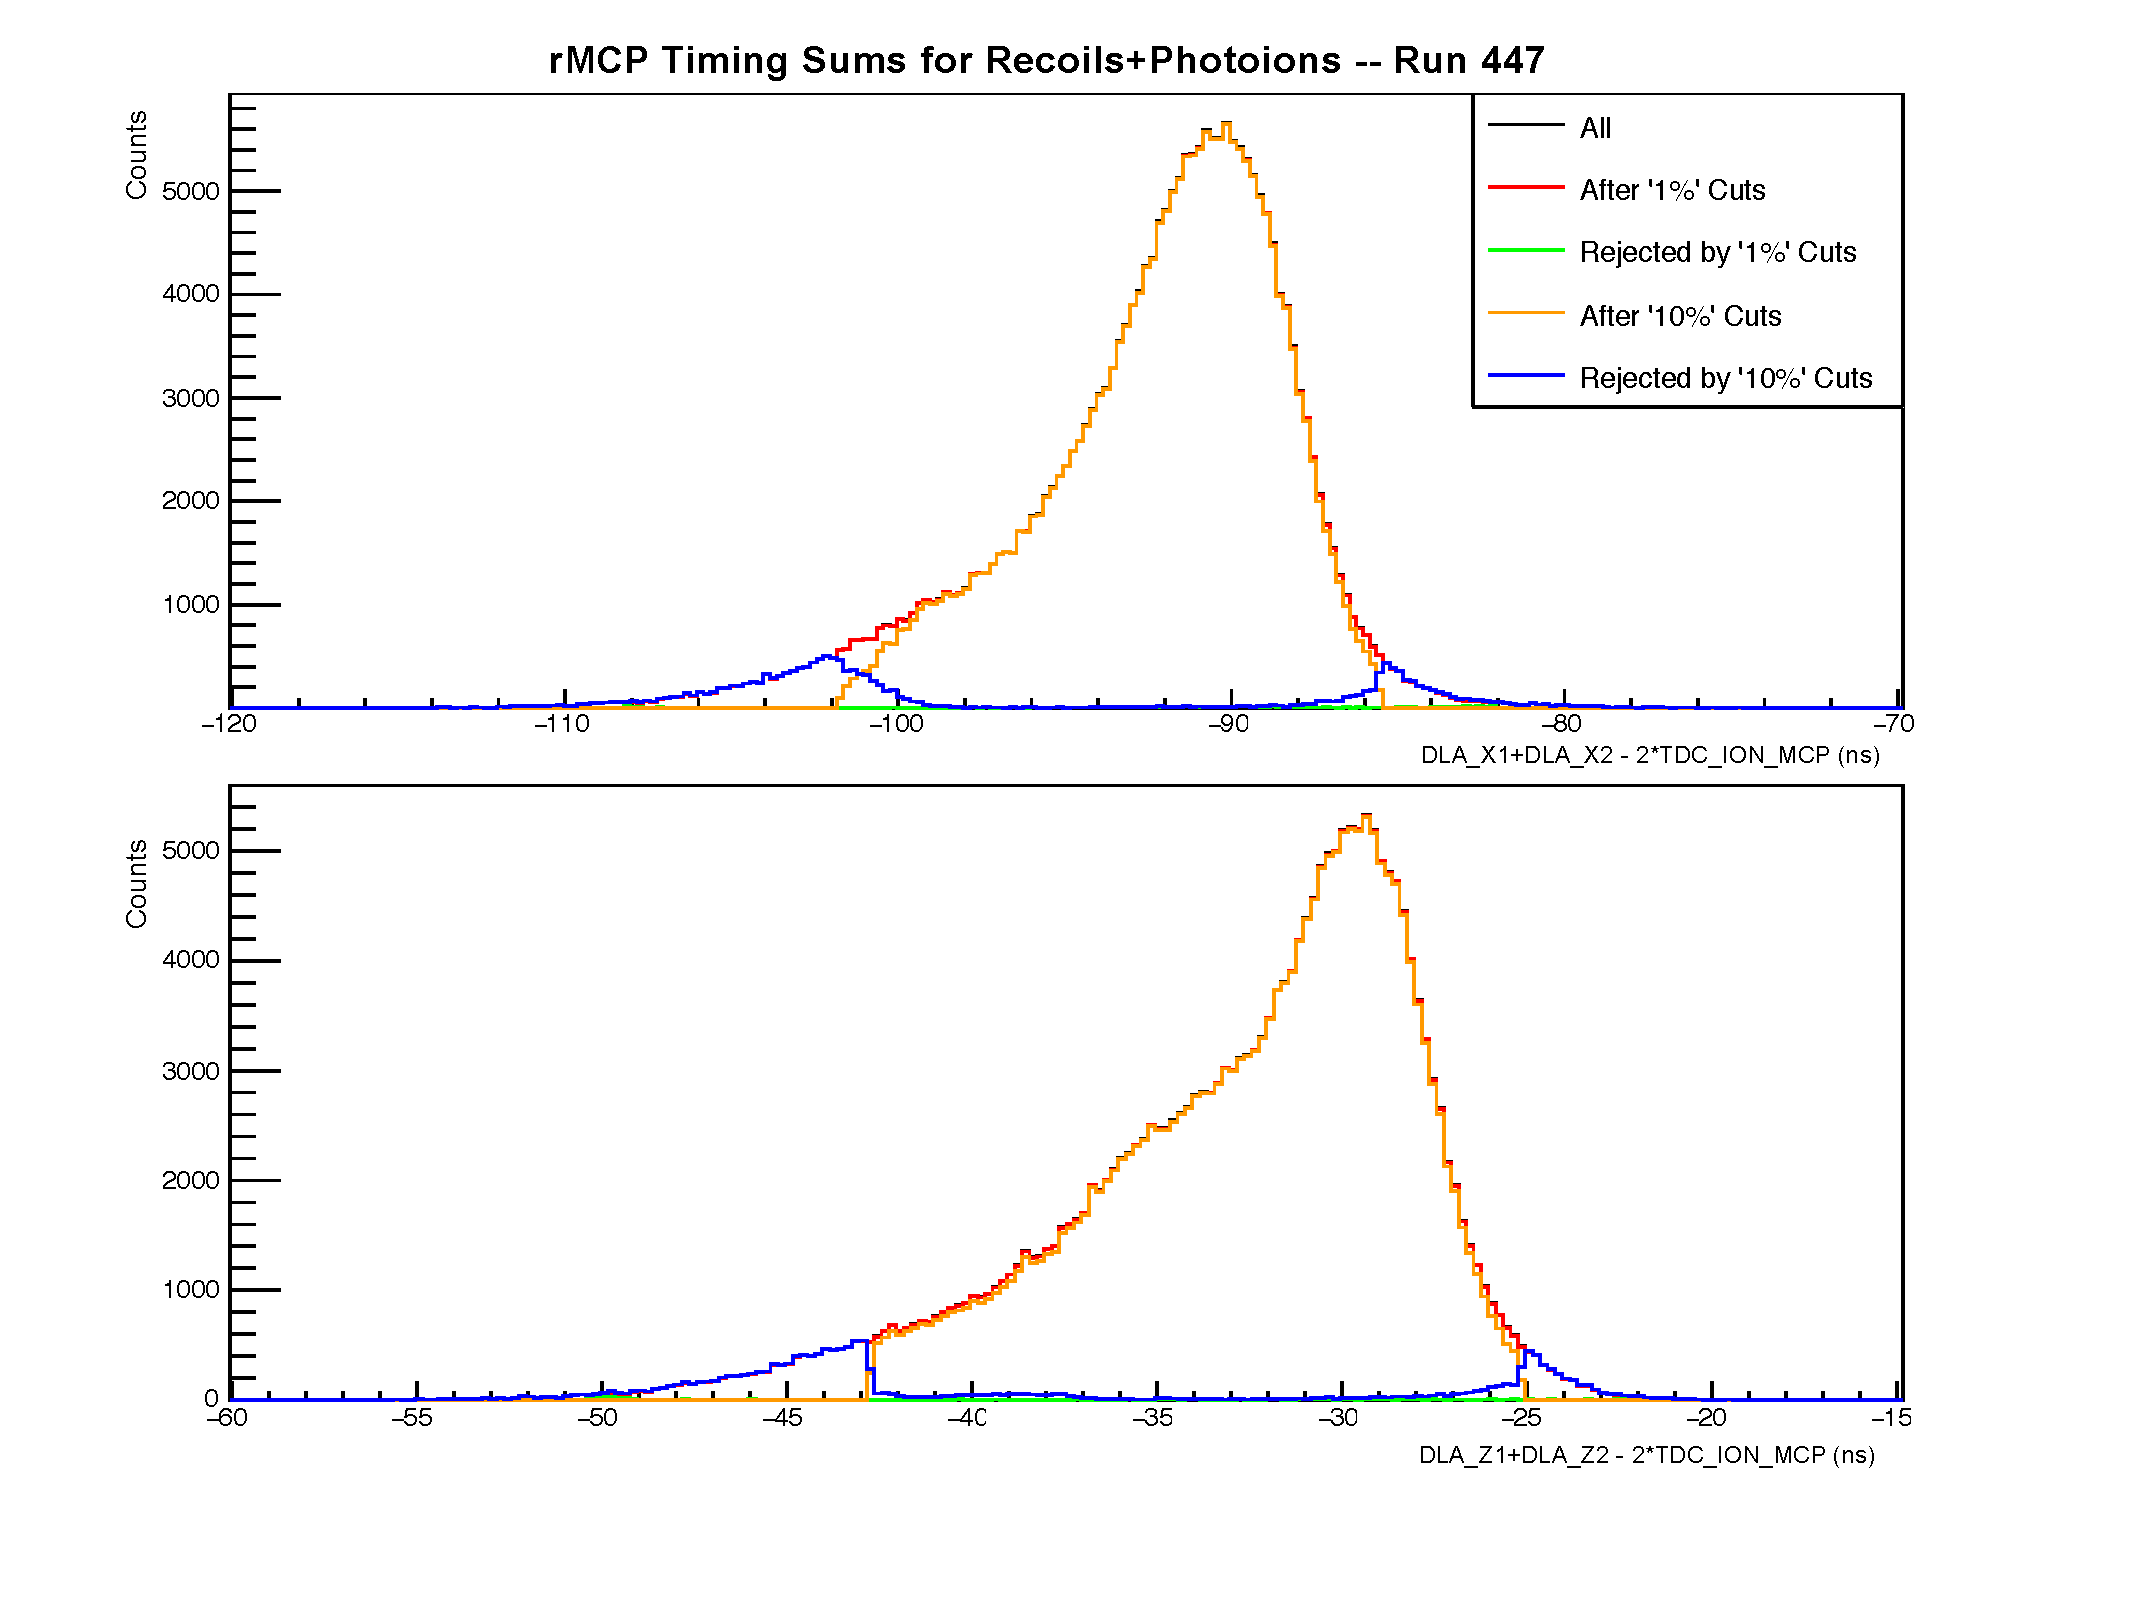
\includegraphics[width=.999\linewidth]
	{Figures/rMCP_sumcuts_447.pdf}
	\note{Are these things *definitely* in nanoseconds?  Check!}
	\note{This algorithm does *not* discard $10\%$ of events!}
	\caption[Timing sums for the rMCP, run 447.]{Timing sums and associated cuts for the rMCP detector, run 447.  The `$10\%$' cuts shown simply eliminate events in which the distribution's height at that value is less than `$10\%$' of that distribution's maximum, and the `$1\%$' cuts are performed in a similar manner.  This figure shows the results after cuts on \emph{both} distributions are taken.   
	%  Only a single run is shown here because the shapes, widths, and positions of these distributions varied significantly over the course of the beamtime, and not all of the changes can be attributed to e.g. a change in settings.  
	}	
	\label{fig:sumcuts}
\end{figure}

Because the characteristics of these timing sum distributions varied from run to run, it didn't make sense to aggregate all the data before taking cuts, so any cuts had to be chosen on a run-by-run basis.  Because of the asymmetry and occasional bimodality of the distributions, it also didn't make sense to try to fit the distributions to a function such as a gaussian and then cut away some number of sigma from the fit function.  The algorithm that was used in the end was to determine the peak's maximum, then discard events from the portion of the distribution in which the distribution's height is less than $10\%$ of the maximum.  

% and it also didn't make sense to try to fit a function such as a gaussian and then cut away some number of sigma from 
%-- so all cuts on the rMCP delay line timing sums had to be taken on a run-by-run basis, and because of the asymmetry and occasional bimodality of the distributions,   
%In particular, we consider the the signals

\section{Calibrations with the rMCP}

\note{This section must be re-phrased.}
Right, so. We removed the mask before the run for some reason (did that happen when we had to open the chamber at the last minute?  I think it was probably actually planned...), so we had to rely on a calibration run we had taken months prior, using a calibration mask.  We only have a single calibration run.  I think we used an alpha source, but maybe I should check on that.  

Using the offline run with the calibration mask, one can see that the lines aren't quite straight.  They're also not necessarily in the spot where they should go, either.  So, I just stretched the image out.  There were several steps in total.  I forget how they all worked.  There was a rotation, and the each row and column was individually stretched so that the line from the mask was put in the position where it was known to actually be located w.r.t. the center of the detector.

\begin{figure}[h!!tb]
	\centering
	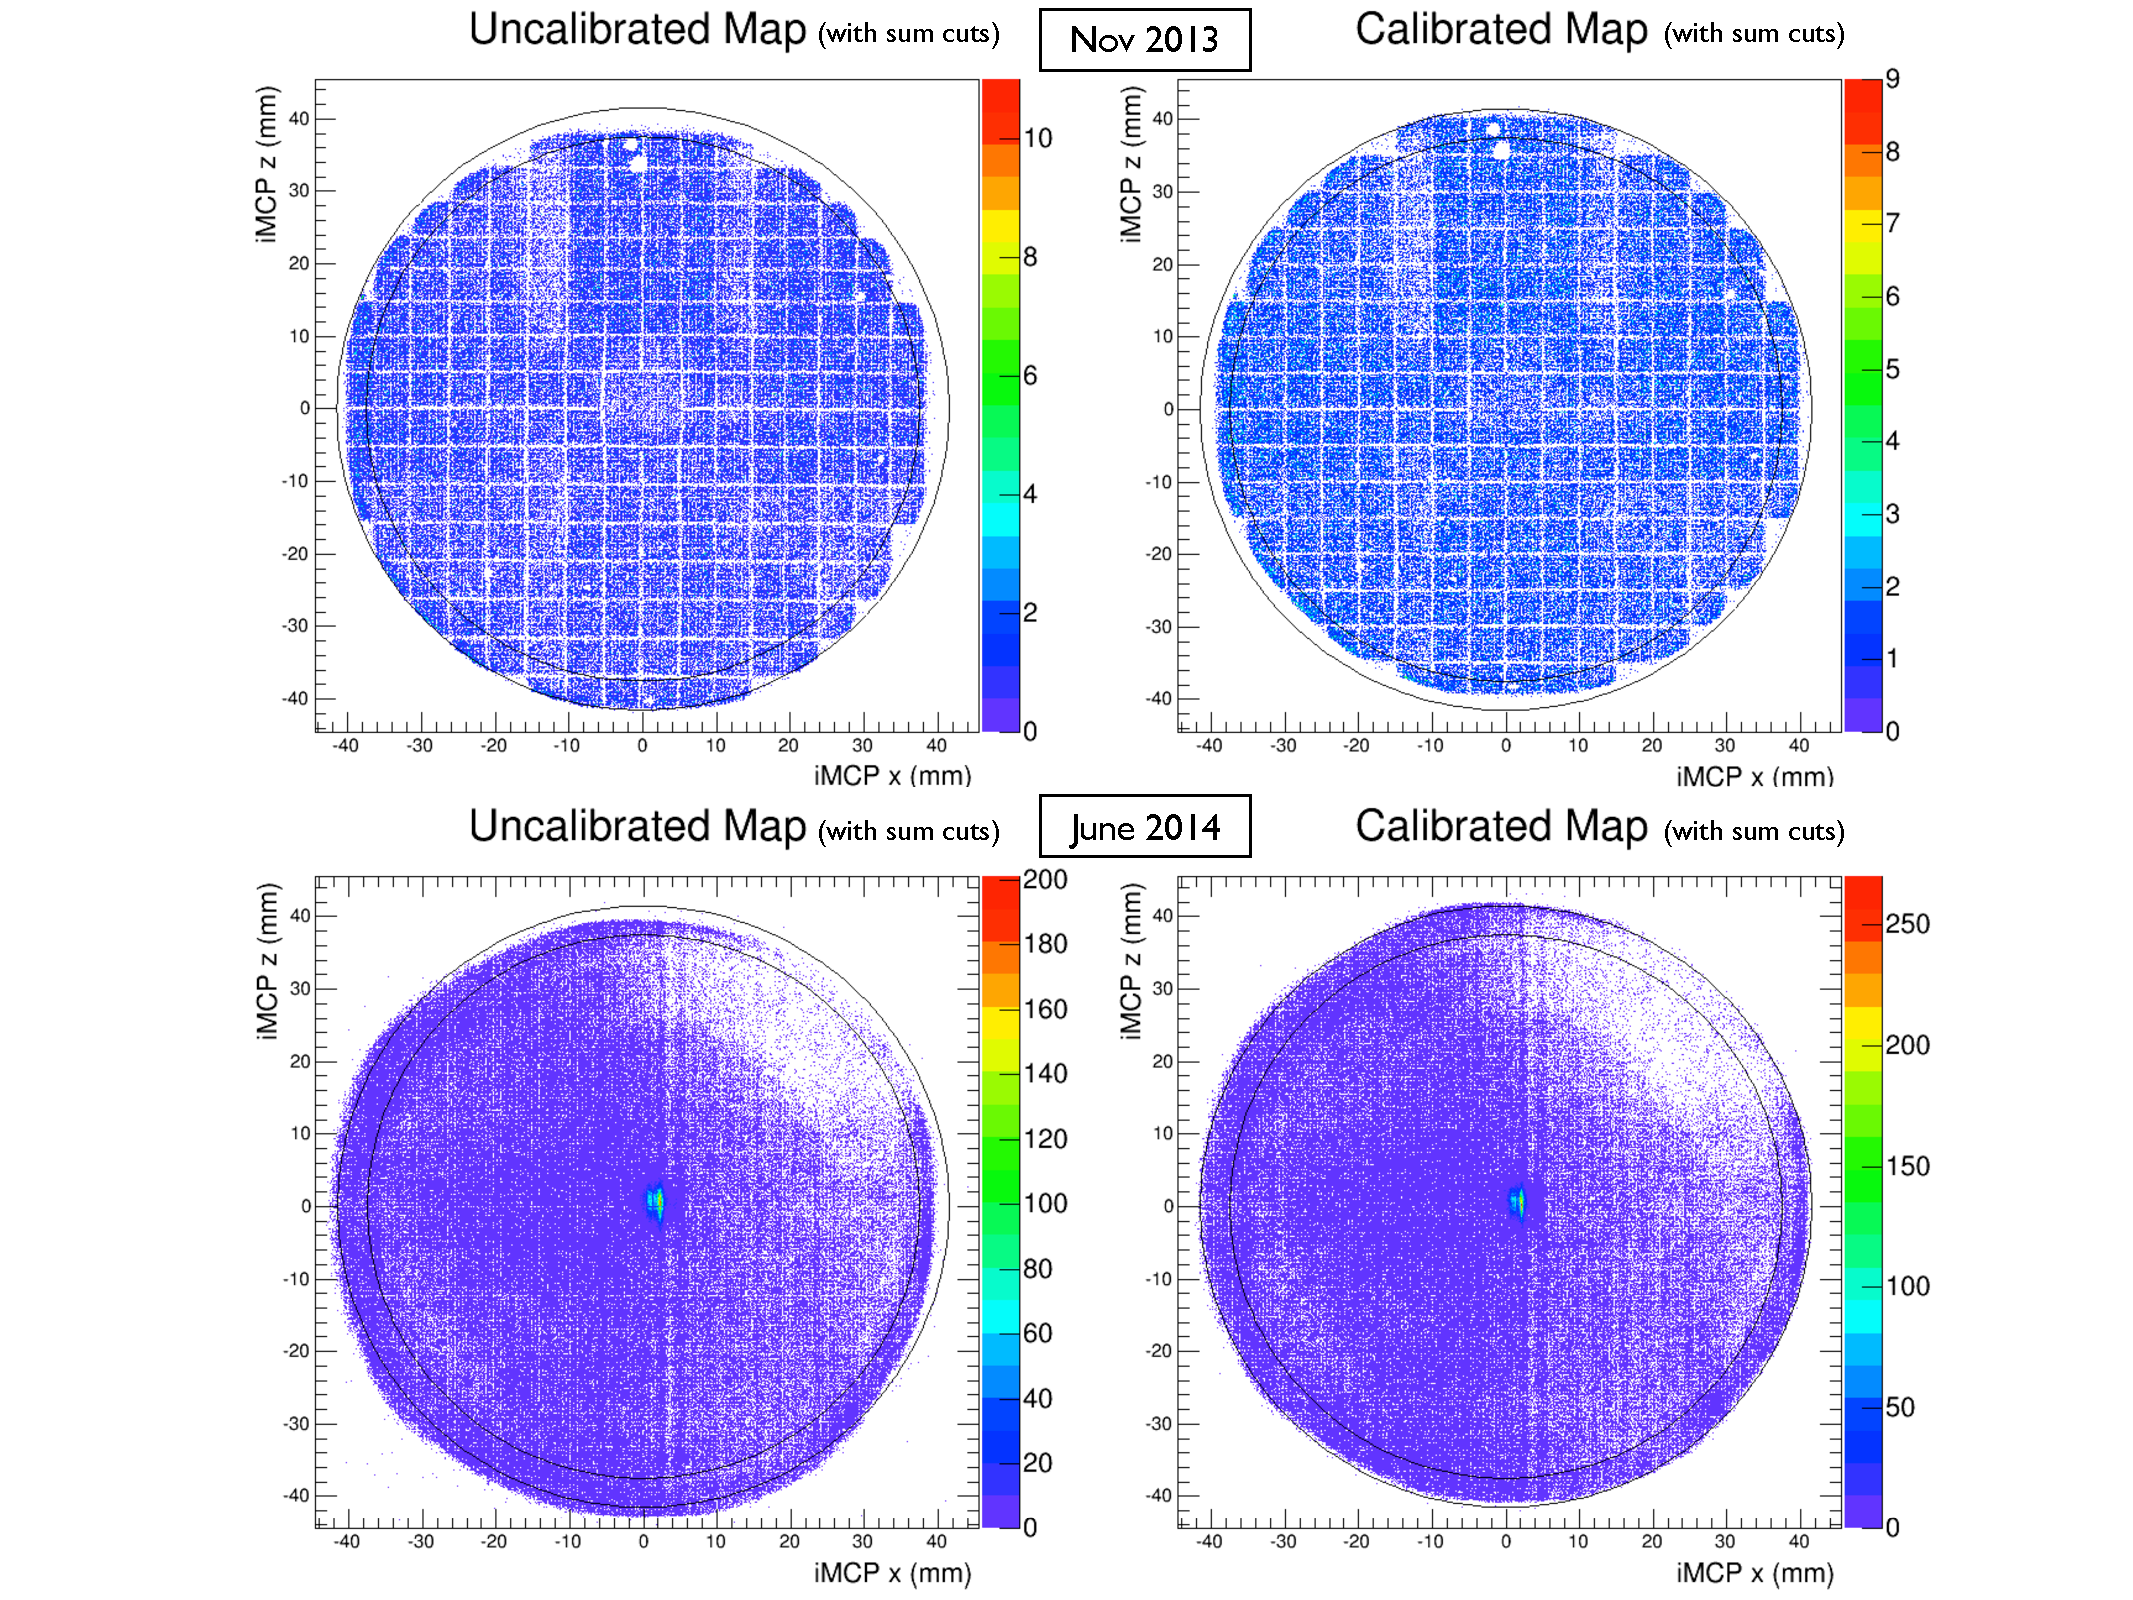
\includegraphics[width=.999\linewidth]
	{Figures/rMCP_Calibration}
	\caption[rMCP Calibration]{rMCP Calibration.  The left images show the rMCP hit map with only a basic preliminary calibration; the images on the right are filled with the same hit data, but after the calibration has been performed.  The upper two images are from data collected offline in advance of the 2014 beamtime using an alpha source; the shadow from a calibration mask is clearly visible.  The lower images show rMCP data taken from a single online run, with the photoion image of the atom cloud visible in the centre.}
	\note{Vertical stripes of seemingly varying gain can be seen on the lower images, as in most of the online rMCP data.  We can't be certain about what caused them, and it has not been possible to eliminate them in analysis.}
	\label{fig:rmcp_calibration}
\end{figure}


The calibration involved:
\begin{itemize}
	\item rotate
	\item cal\_slide
	\item big\_squeeze
	\item micro\_squeeze\_x and micro\_squeeze\_z
	\item edge\_stretch
\end{itemize}



\note{the rMCP does both cloud position *and* cloud polarization, and it collects data faster than the camera can go, so we really kind-of need it for polarization I think?  Except we had that oscilloscope readout too, and that would have basically been fine I think.  Camera does position, but not quickly, so we'd just get an average over all the AC-MOT times or whatever, which isn't really what we want.  Though, turns out that's not a super big systematic anyway.  But whatever, the rMCP is useful, dammit!}

\note{Some kind of segue into a description of what needed to be done to get the rMCP to do what we wanted.}





These calibrations are done during AC-MOT time, and we're actually interested in the rMCP data taken during OP time.  Can I find pictures to estimate the size of the change resulting from the magnetic field?  In any case, the change is pretty small.  

%\subsection{rMCP Bullet Points!}
%	\begin{itemize}
%	\item 
Now, the unsorted bullet points for the rMCP stuff!

	Using the ``other'' data set with the rMCP:  Measure the trap position/size/velocity/expansion with the rMCP and with the camera.  Necessitates calibrating the rMCP, which is its own whole thing.  Also measure polarization.
\begin{itemize}
	%	\item rMCP calibration probably gets its own section, if not its own chapter..
	\item We took the mask off before the 2014 run, to give us more detector area.  Use previous reference calibration \emph{with the mask} during the test run in Nov 2013.  The delay line's non-linearities should be the same, assuming we can get the centering the same.  Cables have changed and stuff, so we have to re-center the pre-calibration image to where the old pre-calibration image was.  ...  So, center the new runs w.r.t the old run.
%		\item We'll want to make some sum cuts for these things.  We might like them to be identical, or at least identical-ish, but the peaks don't really look the same.  So we'll settle for ``decent sum cuts for all!".  ...  So, apply sum cuts to the new runs and old run.
%		\item Calibrate the old run, with the mask.  In fact, I don't remember which order I did things in.  But I have a record of it here, somewhere...
\end{itemize}



%I really need an excuse to include more pictures of data.  Also, more pictures of simulations.
Without further ado, I'm just going to put in several pictures.  Right here, right now.  They're likely to *actually* show up on subsequent pages mixed in with the other content.  I'll have to fix that at some point.
\begin{figure}[h!!t]
	\centering
	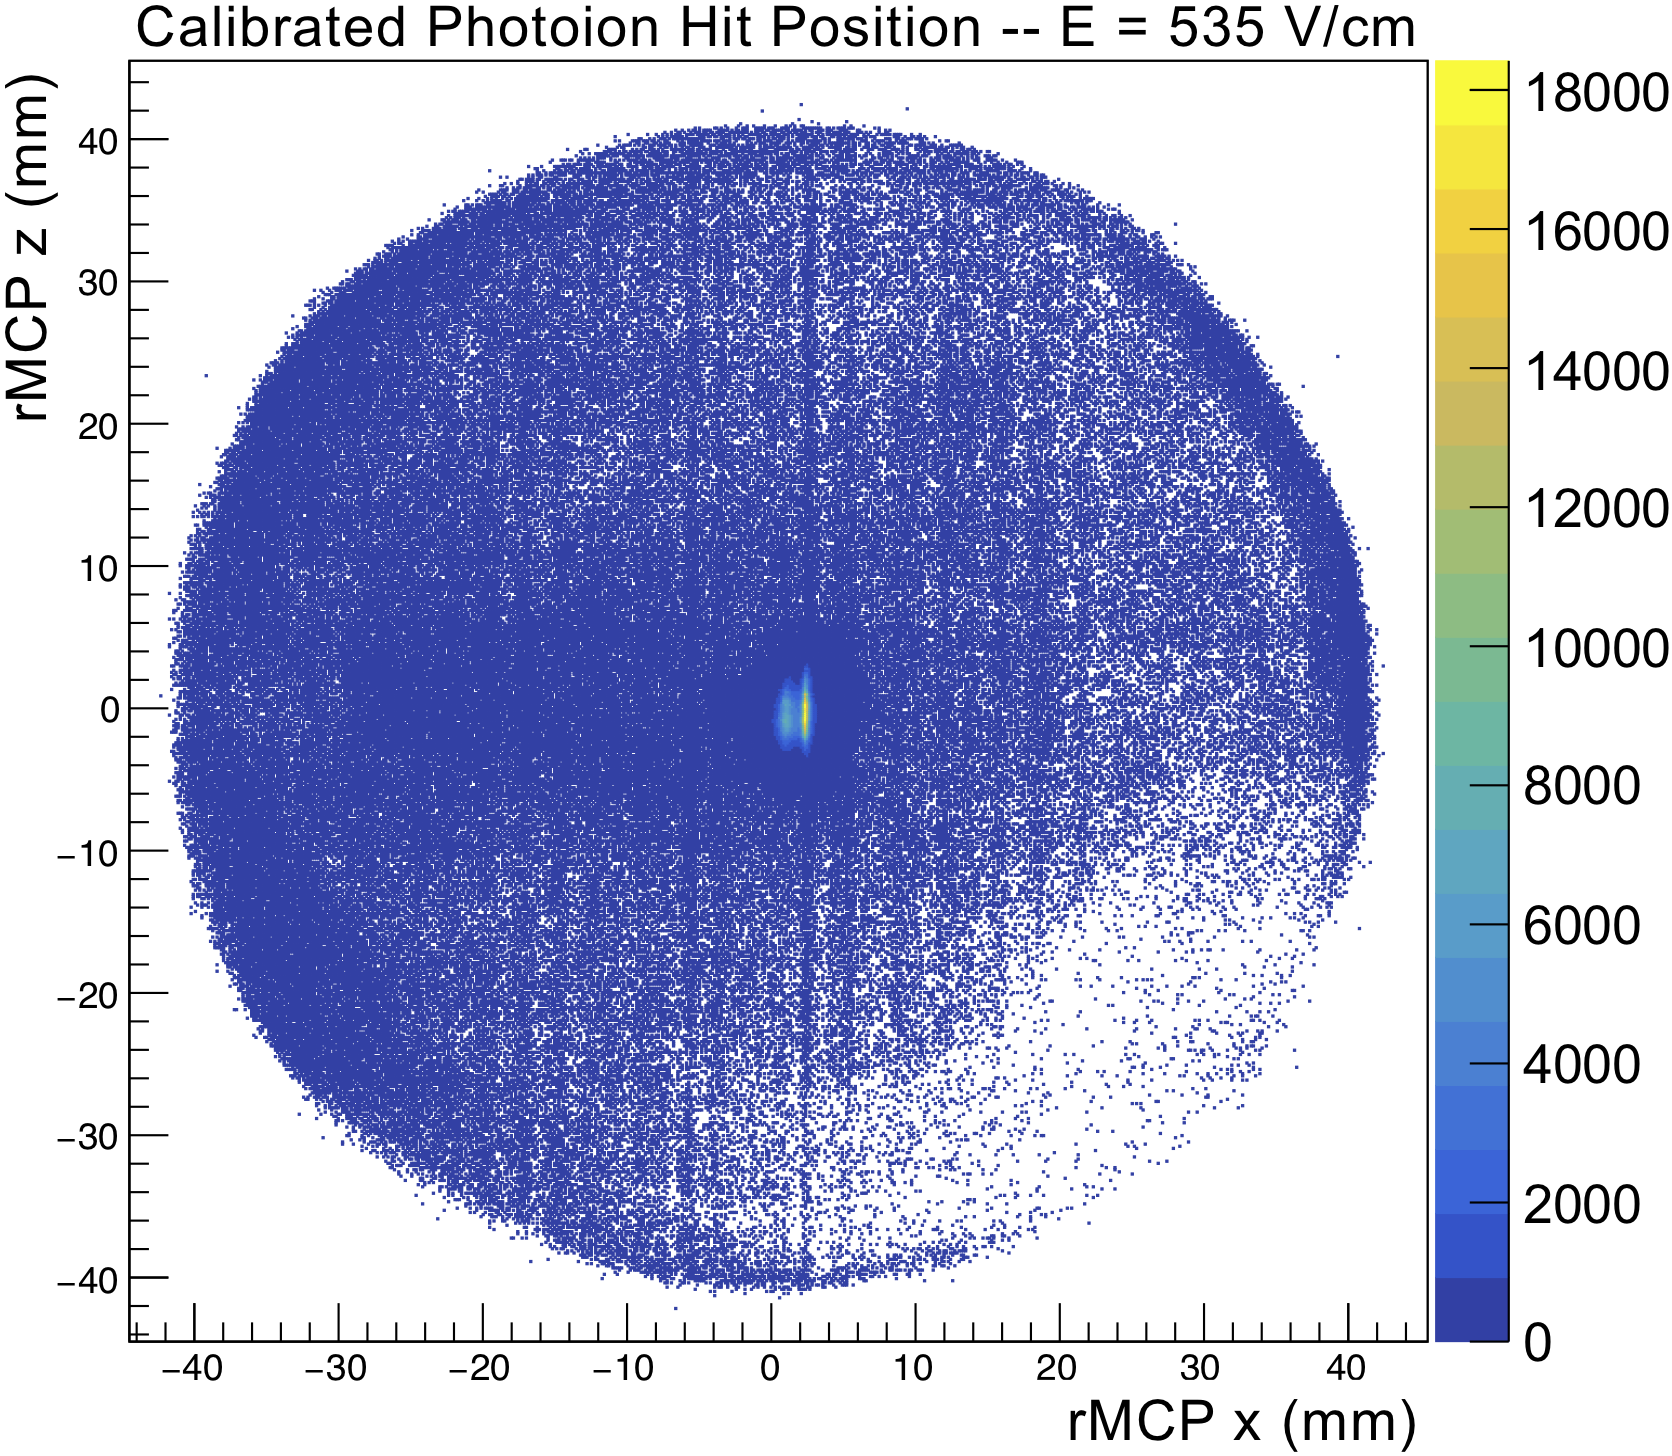
\includegraphics[width=.999\linewidth]
	{Figures/rMCP_PI_2D_535.png}
	\note{This figure needs to be discussed in text or whatever.}
	\caption[Photoion Hit Positions in 2D]{Photoion Hit Positions in 2D.  This is all of the data taken at 535 V/cm.}	
%	\label{fig:vposition_by_run_rmcp}
\end{figure}
\begin{figure}[h!!t]
	\centering
	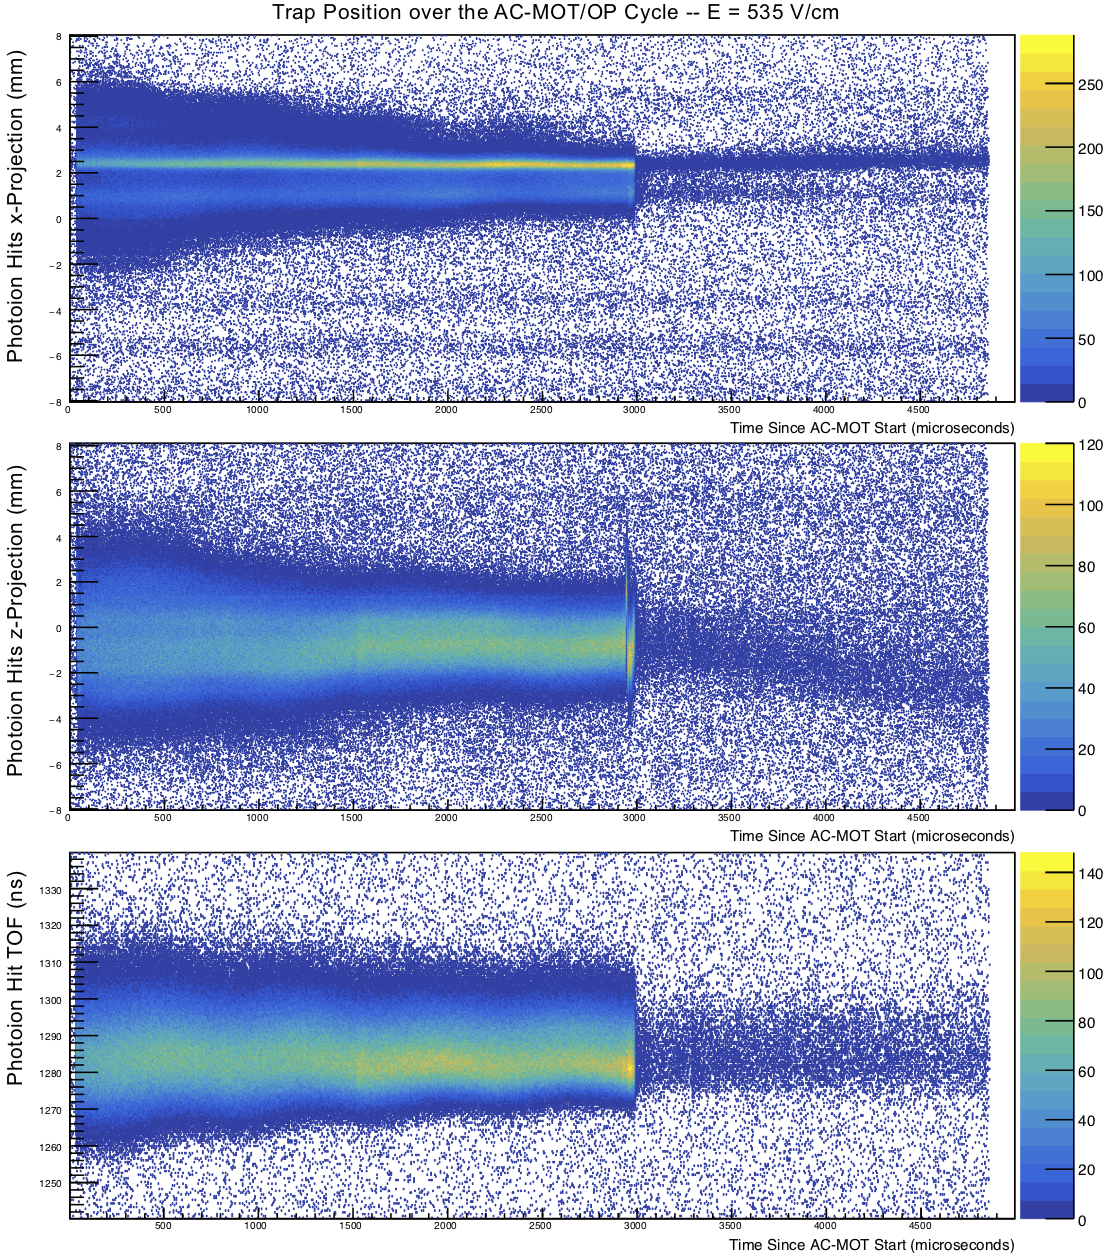
\includegraphics[width=.999\linewidth]
	{Figures/rMCP_xyz_vs_acmottime.png}
	\note{This figure needs to be discussed in text or whatever.}
	\caption[Photoion Hit Positions at 535 V/cm, as a function of AC-MOT Time]{Photoion Hit Positions at 535 V/cm, as a function of AC-MOT Time}	
%	\label{fig:vposition_by_run_rmcp}
\end{figure}
\begin{figure}[h!!t]
	\centering
	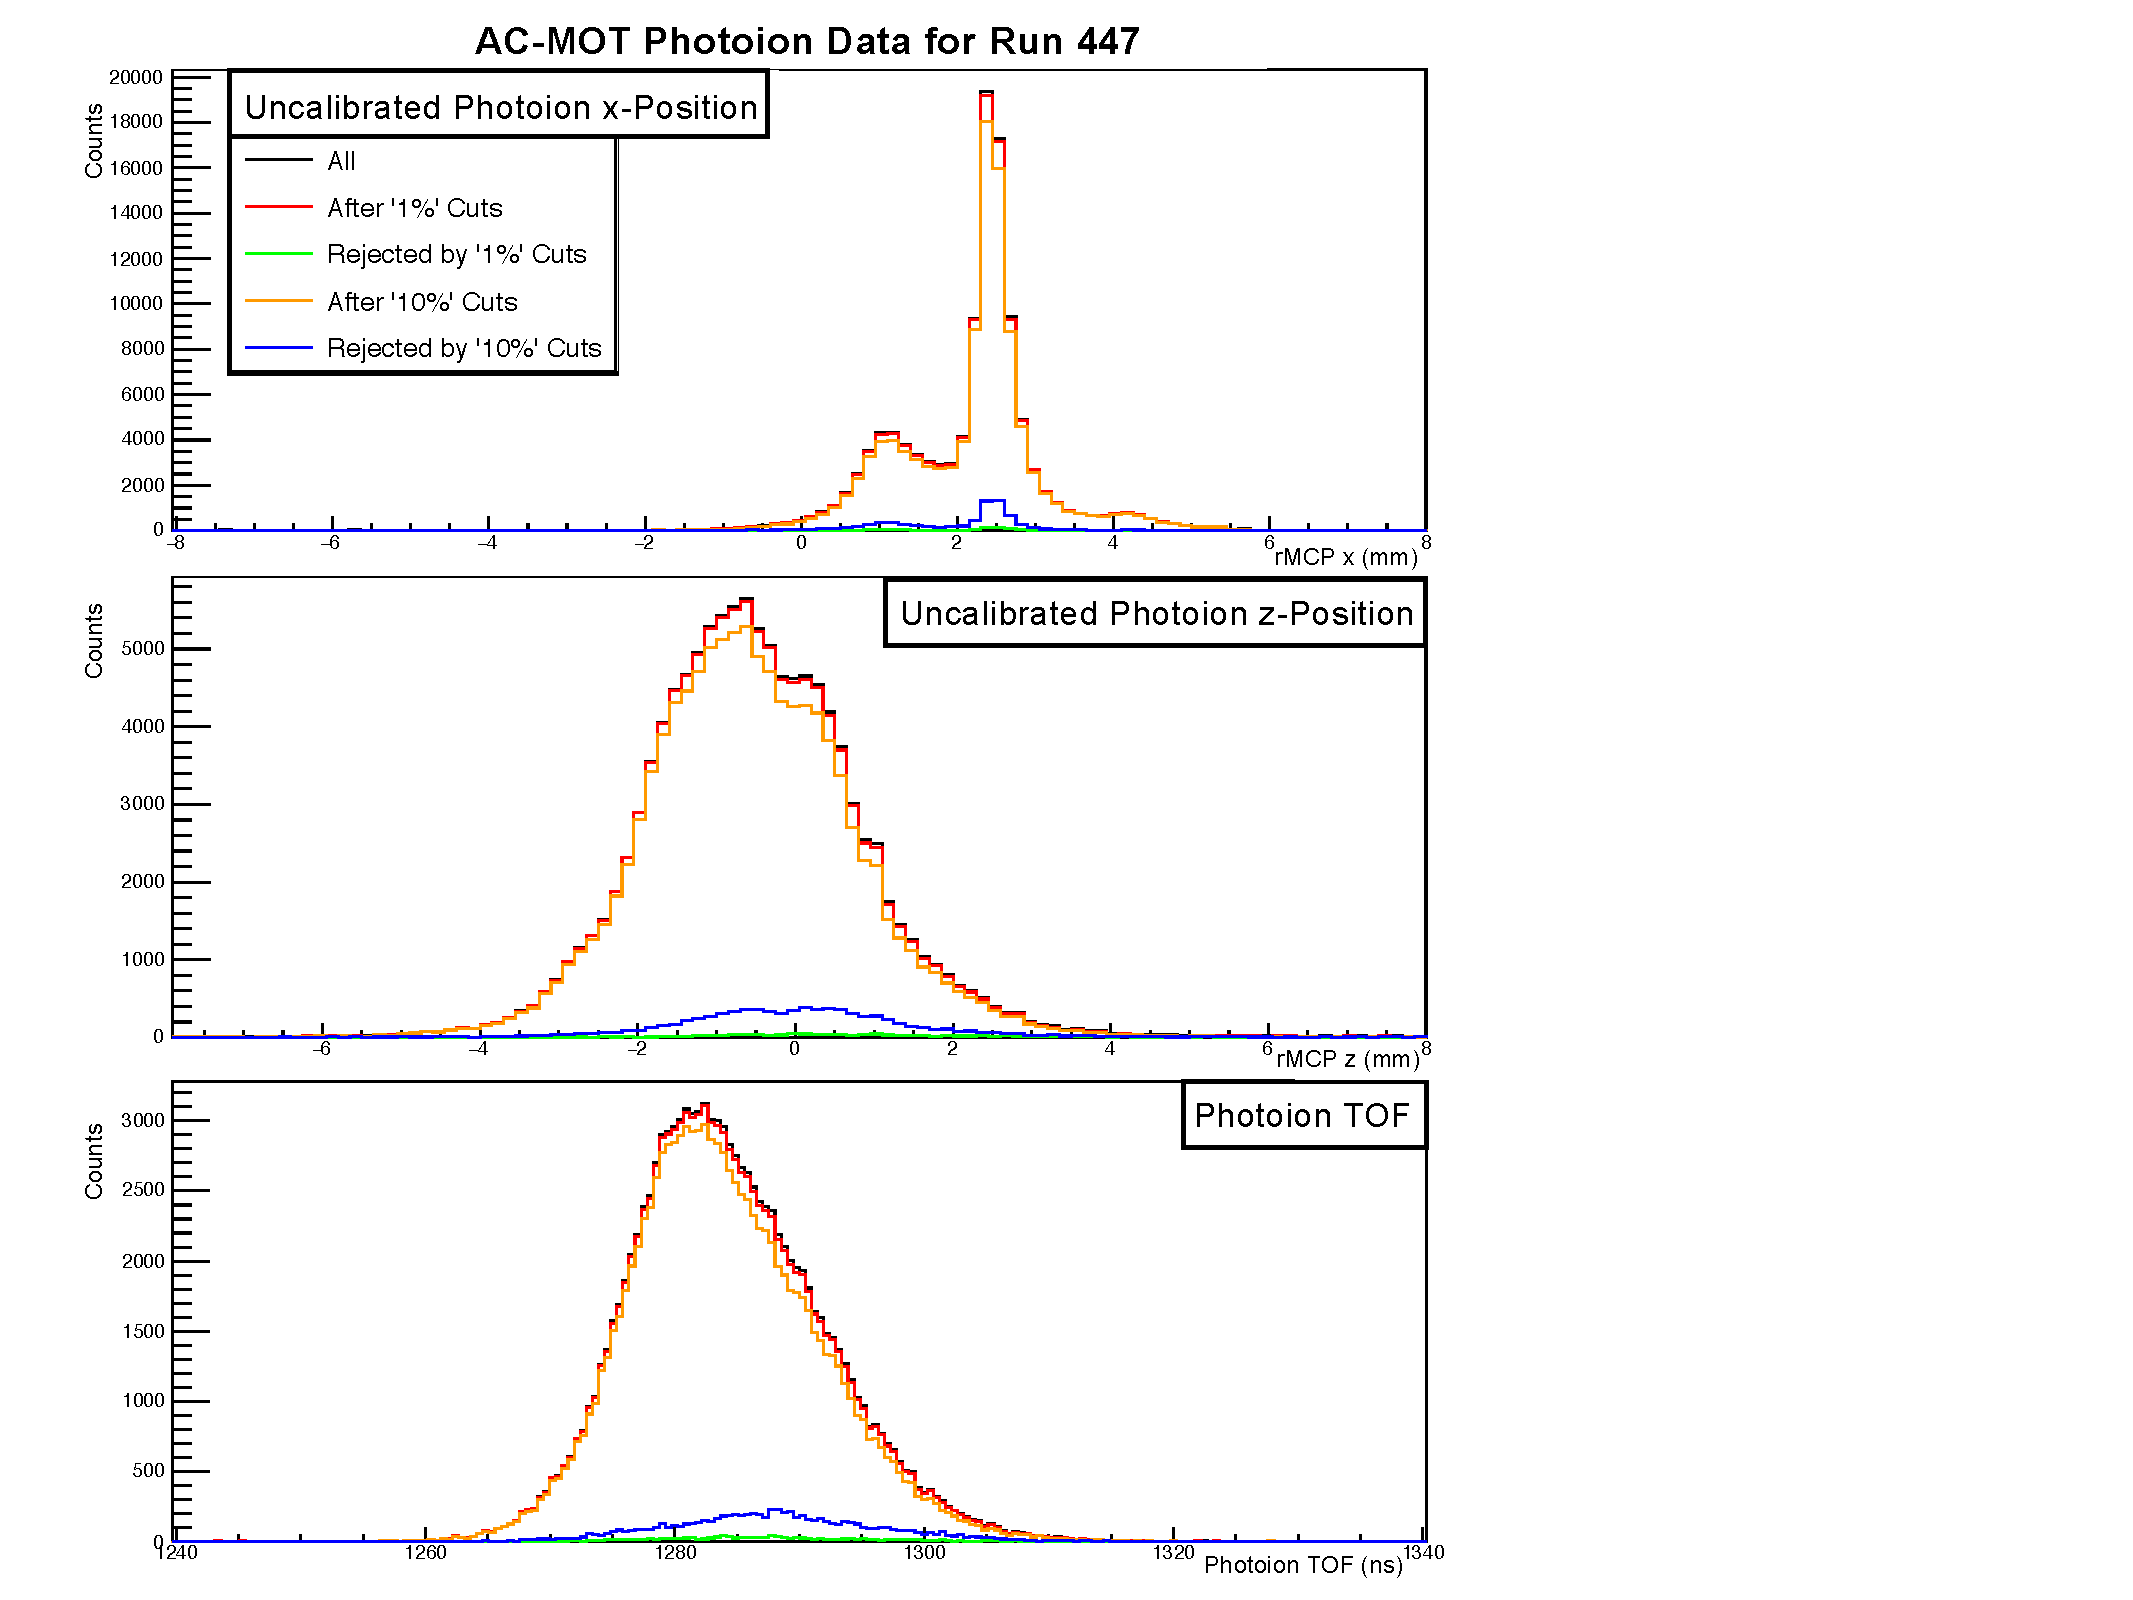
\includegraphics[width=.999\linewidth]
	{Figures/rMCP_xyz_comparecuts447.pdf}
	\note{This figure needs to be discussed in text or whatever.}
	\caption[A projection along all three axes for run 447, with various cuts on the rMCP delay line timing sum.]{A projection along all three axes for run 447, with various cuts on the rMCP delay line timing sum.}	
%	\label{fig:vposition_by_run_rmcp}
\end{figure}




\note[color=org]{I have some tables summarizing which types of data were measured.  Presently, that's in Ch-4 (now ch.3), but probably I should move it here.}
\label{calibrations_chapter}

\section{Measurements of the Atom Cloud}
\label{sec:cloud_calibration}
\note{Pretty sure this section needs to be merged with the previous section on rMCP measurements.}

\note[color=org]{Content that previously was in this subsection is now in Section~\ref{cloud}.  But also, see the section about the photoionization laser.  Probably in this section here, I need to just jump right in assuming everyone understands the physical principle of how the data works.  Then, I can talk about what the data *is*, and how it gets interpreted.}

%\label{cloud}
%\label{photoions}
%\note[color=org]{Some of this stuff is in Ch.3 and/or Ch.4.  Some of it *should* be.}
%In order to measure properties of the trapped $^{37}\textrm{K}$ cloud, a 10\,kHz pulsed laser at 355\,nm is directed towards the cloud.  These photons have sufficient energy to photoionize neutral $^{37}\textrm{K}$ from its excited atomic state, which is populated by the trapping laser when the MOT is active, releasing 0.77\,eV of kinetic energy, but do not interact with ground state $^{37}\textrm{K}$ atoms.  The laser is of sufficiently low intensity that the great majority\aside[color=jb]{JB:  ``On order 1\% are photoionized."} of excited state atoms are \emph{not} photoionized, so the technique is only very minimally destructive.  
%\note{Probably worth mentioning that we test this stuff offline on stable \isotope[41]{K}. }
%
%
%Because an electric field has been applied within this region (see Section~\ref{field})\aside[color=jb]{JB:  ``you could reference the letter for the value of the field 150V/cm.''} the $^{37}\textrm{K}^+$ ions are immediately pulled into the detector on one side of the chamber, while the freed $e^-$ is pulled towards the detector on the opposite side of the chamber.  Because  $^{37}\textrm{K}^+$ is quite heavy relative to its initial energy, it can be treated as moving in a straight line directly to the detector, where its hit position on the microchannel plate is taken as a 2D projection of its position within the cloud.  Similarly, given a sufficient understanding of the electric field, the time difference between the laser pulse and the microchannel plate hit allows for a calculation of the ion's initial position along the third axis.  
%
%\note{As a check:  the camera measurements for photons from de-excitation.  It's aimed 35 degrees from vertical, with its horizontal axis the same as ..... one of the other axes.  I think it's the TOF axis.  I can check this when my computer comes back.   Also, there's an unknown additional delay between some of our DAQ channels that can't be explained by accounting for cable lengths, so we really like having the check there.}
%\note[color=jb]{JB says:  ``yes, camera x-axis is tof axis.''}
%
%
%With this procedure, it is possible to produce a precise map of the cloud's position and size, both of which are necessary for the precision measurements of angular correlation parameters that are of interest to us here.  However, it also allows us to extract a third measurement:  the cloud's polarization.
%
%The key to the polarization measurement is that only atoms in the excited atomic state can be photoionized via the 355 nm laser.  While the MOT runs, atoms are constantly being pushed around and excited by the trapping lasers, so this period of time provides a lot of information for characterizing the trap size and position.  When the MOT is shut off, the atoms quickly return to their ground states and are no longer photoionized until the optical pumping laser is turned on.  As described in Section~\ref{op}, and in greater detail in~\cite{ben_OP}, the optical pumping process involves repeatedly exciting atoms from their ground states until the atoms finally cannot absorb any further angular momentum and remain in their fully-polarized (ground) state until they are perturbed.  Therefore, there is a sharp spike in excited-state atoms (and therefore photoions) when the optical pumping begins, and none once\aside[color=jb]{JB points out that this should be ``if", not ``once".} the cloud has been completely polarized.  The number of photoion events that occur once the sample has been maximally polarized, in comparison with the size and shape of the initial spike of photoions, provides a very precise characterization of the cloud's final polarization~\cite{ben_OP}.



\note{Trap position -- Measured using the same dataset that was used to quantify the polarization.  The trap drifts slightly over the course of our data collection.  Describe the rMCP calibration needed to extract this info.}
\note{Polarization measurement was conducted on a different set of data, collected in between the measurements used for $A_{\mathrm{\beta}}$ and $b_{\mathrm{Fierz}}$, and at a higher electric field, because we were unable to run both our MCP detectors simultaneously.  }

\missingfigure{Need pictures of the cloud.  Possibly need projections of the cloud as a function of time, for AC/OP cycles.}
%\note{Need to describe how polarization works.  Needs a level diagram.  Needs another(?) level diagram for the photoionization, and maybe a third for the MOT.  Can I combine them all?  idk.}

Anyway, here is a nice table describing the atom cloud, for each of 3 runsets, and I'll immediately reference it right now, as Table~\ref{table:cloudpositions}:

% !TEX root = ../thesis_main.tex


\begin{table}[h!!!!t]
	\begin{center}
	\begin{tabular}{ c | r || lcl | lcl || lcl | lcl |}
	%	\hline
	%		\multicolumn{5}{ | c | }{Cloud Measurements -- $x$-Projection} \\
	%	\hline\hline
	%	\cline{3-6}
			\multicolumn{2}{  c  }{ } & 
				\multicolumn{3}{  c  }{ \!\!Initial Position\!\! } &  \multicolumn{3}{   c  }{ Final Position } &  \multicolumn{3}{   c  }{ Initial Size } &  \multicolumn{3}{   c  }{ Final Size } \\
		%	\cline{2-6}
		%	\hline
		%	\cline{2-6}
			\cline{2-14}
			\multirow{3}{*}{Runset B}  & $x$ & \,\,1.77 & \!\!$\!\! \pm  \!\!$\!\! & 0.03   & \,\,2.06   & \!\!$\!\! \pm  \!\!$\!\! & 0.08    & 0.601 & \!\!$\!\! \pm  \!\!$\!\! & 0.013 & 1.504 & \!\!$\!\! \pm  \!\!$\!\! & 0.047 \\
								& $y$ & -3.51    & \!\!$\!\! \pm  \!\!$\!\! & 0.04   & -3.33     & \!\!$\!\! \pm  \!\!$\!\! & 0.05    & 1.009 & \!\!$\!\! \pm  \!\!$\!\! & 0.013 & 1.551 & \!\!$\!\! \pm  \!\!$\!\! & 0.018 \\
								& $z$ & -0.661  & \!\!$\!\! \pm  \!\!$\!\! & 0.005 & -0.551   & \!\!$\!\! \pm  \!\!$\!\! & 0.021  & 0.891 & \!\!$\!\! \pm  \!\!$\!\! & 0.004 & 1.707 & \!\!$\!\! \pm  \!\!$\!\! & 0.015 \\
			\cline{2-14}
			\multirow{3}{*}{Runset C}  & $x$ & \,\,2.22  & \!\!$\!\! \pm  \!\!$\!\! & 0.05  & \,\,2.33   & \!\!$\!\! \pm  \!\!$\!\! & 0.11    & 1.18   & \!\!$\!\! \pm  \!\!$\!\! & 0.04   & 1.538 & \!\!$\!\! \pm  \!\!$\!\! & 0.087 \\
								& $y$ & -3.68     & \!\!$\!\! \pm  \!\!$\!\! & 0.04  & -3.31      & \!\!$\!\! \pm  \!\!$\!\! & 0.06   & 0.965 & \!\!$\!\! \pm  \!\!$\!\! & 0.012 & 1.460 & \!\!$\!\! \pm  \!\!$\!\! & 0.030 \\
								& $z$ & -0.437   & \!\!$\!\! \pm  \!\!$\!\! & 0.09  & -0.346    & \!\!$\!\! \pm  \!\!$\!\! & 0.037 & 0.927 & \!\!$\!\! \pm  \!\!$\!\! & 0.007 & 1.797 & \!\!$\!\! \pm  \!\!$\!\! & 0.026 \\
			\cline{2-14}
			\multirow{3}{*}{Runset D}  & $x$ & \,\,2.274 & \!\!$\!\! \pm  \!\!$\!\! & 0.012 & \,\,2.46 & \!\!$\!\! \pm  \!\!$\!\! & 0.06   & 0.386 & \!\!$\!\! \pm  \!\!$\!\! & 0.016 & 1.382 & \!\!$\!\! \pm  \!\!$\!\! & 0.046 \\
								& $y$ & -4.54      & \!\!$\!\! \pm  \!\!$\!\! & 0.04   & -4.28    & \!\!$\!\! \pm  \!\!$\!\! & 0.04   & 0.986 & \!\!$\!\! \pm  \!\!$\!\! & 0.08   & 1.502 & \!\!$\!\! \pm  \!\!$\!\! & 0.013 \\
								& $z$ & -0.587    & \!\!$\!\! \pm  \!\!$\!\! & 0.04   & -0.481  & \!\!$\!\! \pm  \!\!$\!\! & 0.018 & 0.969 & \!\!$\!\! \pm  \!\!$\!\! & 0.003 & 1.861 & \!\!$\!\! \pm  \!\!$\!\! & 0.013 \\
			\cline{2-14}
	\end{tabular}
	\end{center}
%	\label{table:cloudpositions}
	\note{These positions are for the *electron* runsets of those names.  Might want a chart of which rMCP runs are used to measure position for which eMCP runs.  Possibly in that other section.}
	\note{Sig figs here need work.}
	\caption[Cloud Position and Size]{Cloud Positions and Sizes -- Measured immediately before and immediately following the optical pumping phase of the trapping cycle.  All entries are expressed in units of mm, and the ``size" parameters describe the gaussian width.}
	\label{table:cloudpositions}
\end{table}




\note{Also, we noticed the trap drifting after one of the runs, because one of the batteries on one of the thingies adjusting the laser frequency (I think) was failing. }
\note[color=jb]{JB:  ``If we rejected the data with the MOT moving (indeed a battery determining the voltage controlled oscillator frequency offset between absorption in stable \isotope[41]{K} cell and the \isotope[37]{K} resonance) then that's all you need to say.''}
\note{describe how you'd turn this into a physical description of the cloud, with like a temperature and a sail velocity and shit.  with equations.}



\begin{figure}[h!!t]
	\centering
	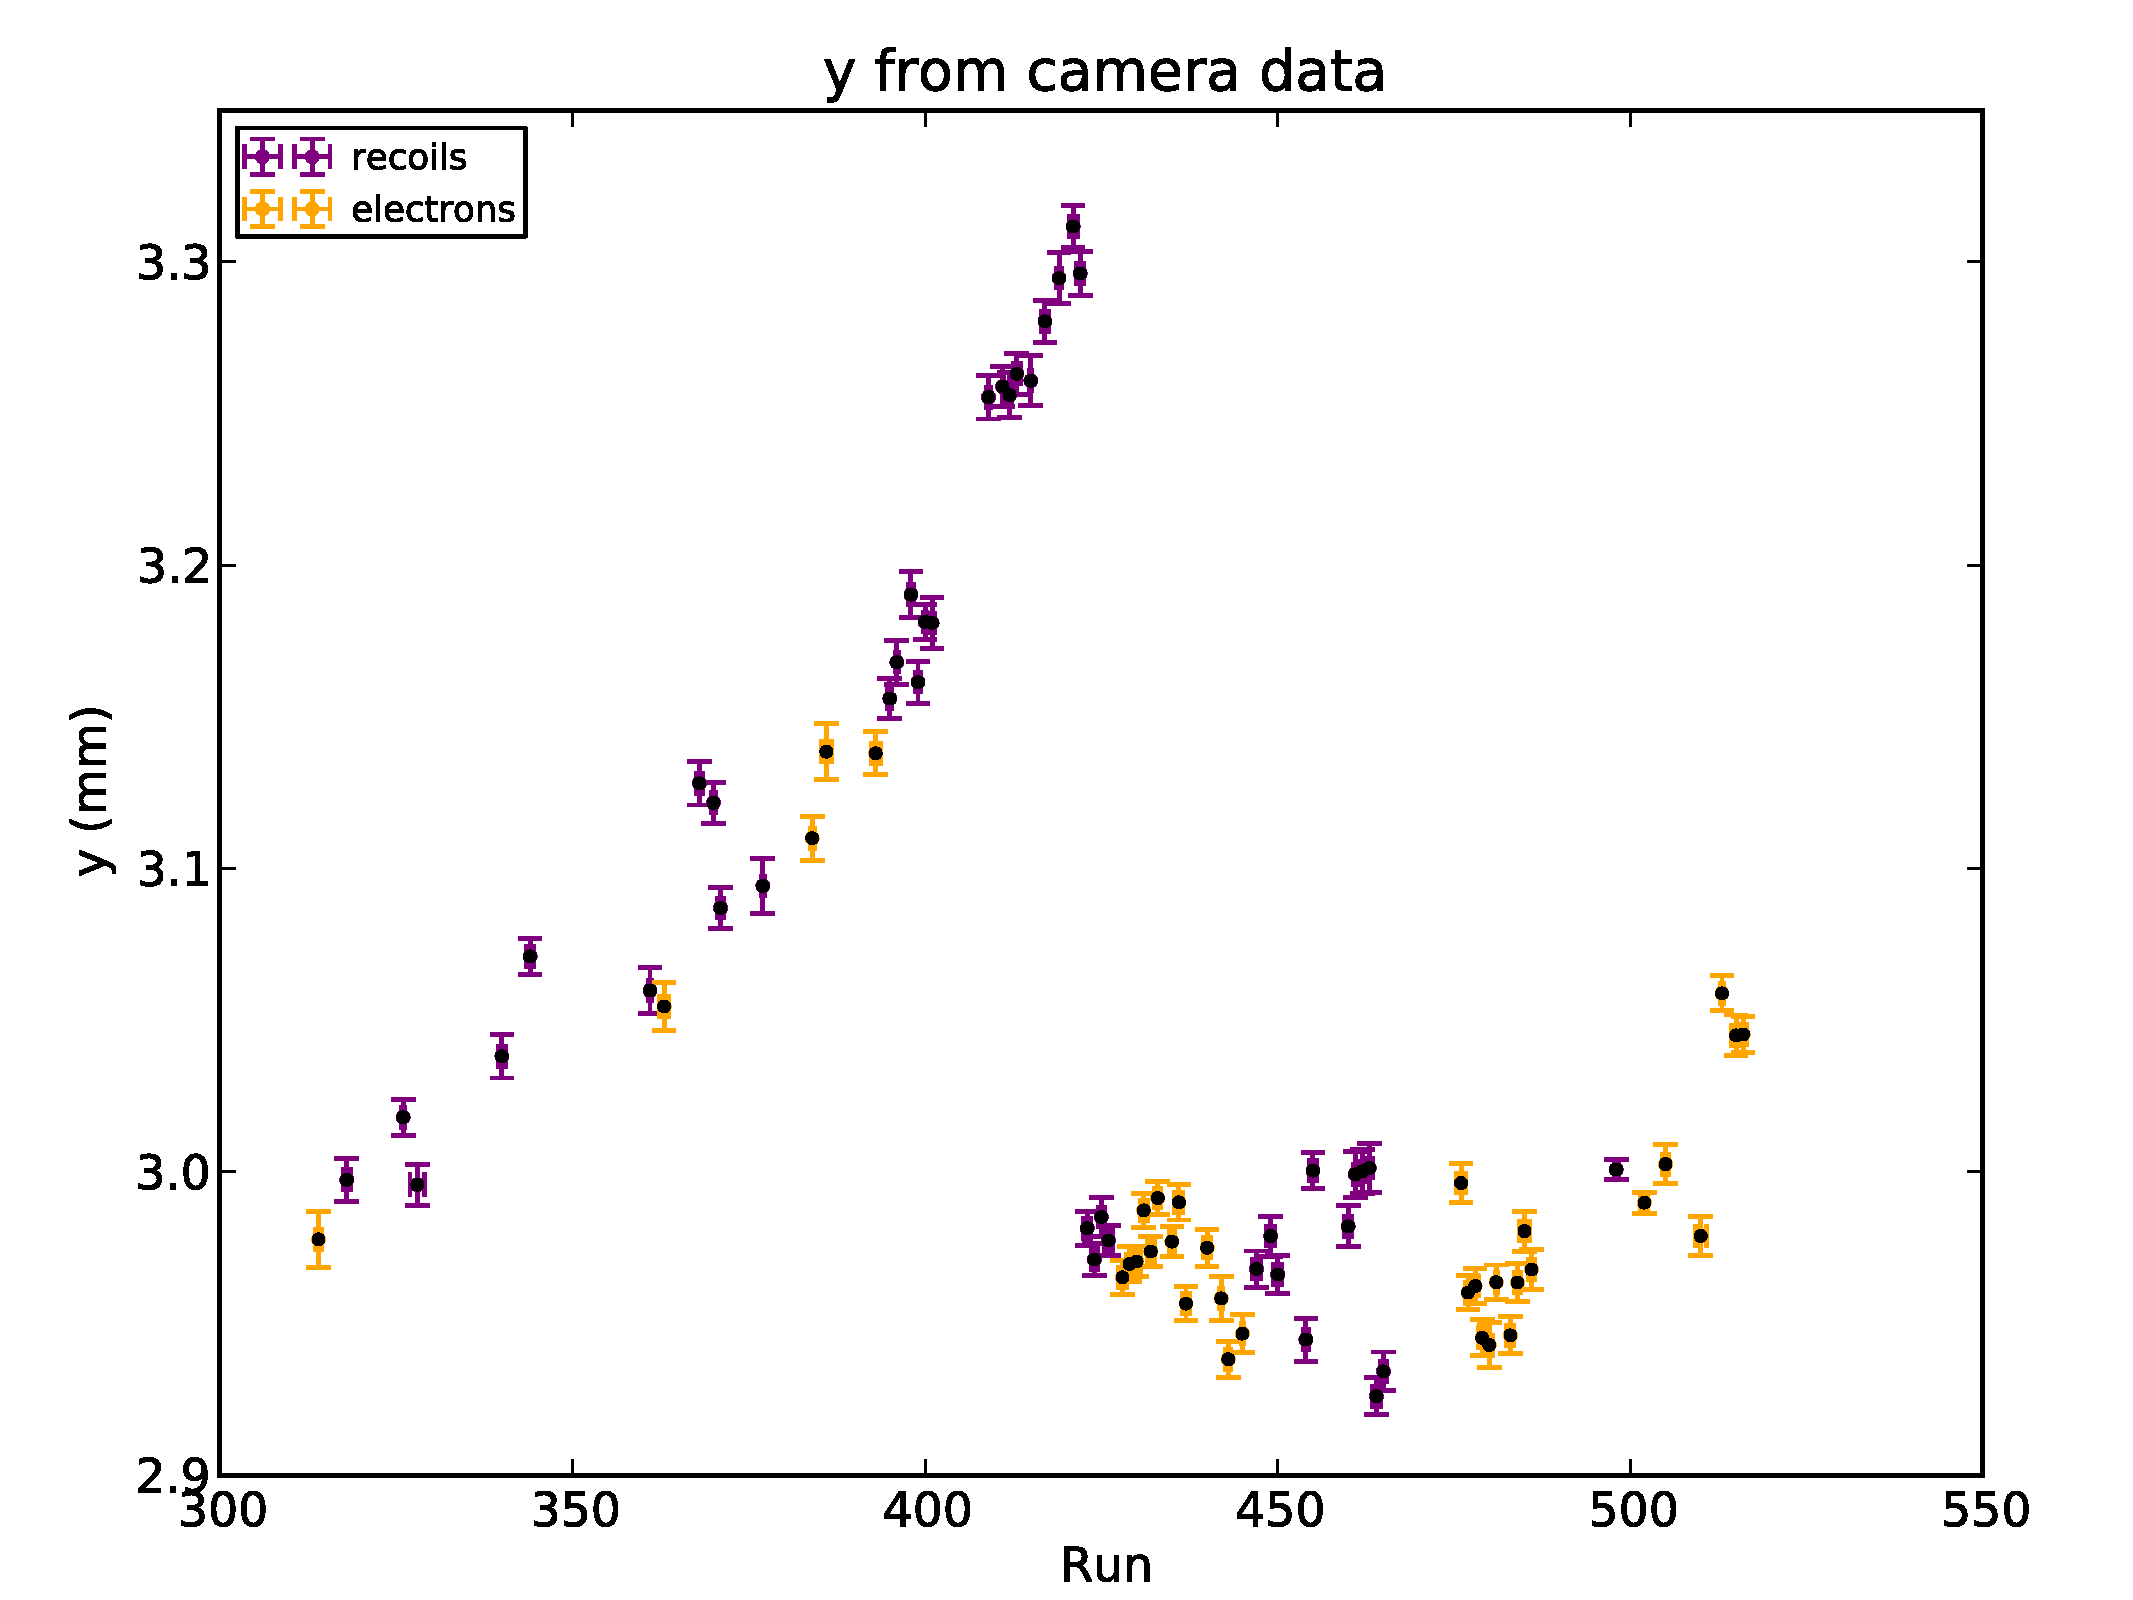
\includegraphics[width=.999\linewidth]
	{Figures/y_from_camera_electron_recoil.pdf}
	\caption[Trap Position along TOF Axis]{Trap Position along the ``Time-of-Flight'' Axis.  Electron runs and recoil runs plotted by run number. \comment{(I should probably re-plot this.  Maybe combine info with Fig.~(\ref{fig:cameraposition_by_time}).) } }	
	\label{fig:camera_electron_recoil}
\end{figure}

\begin{figure}[h!!t]
	\centering
	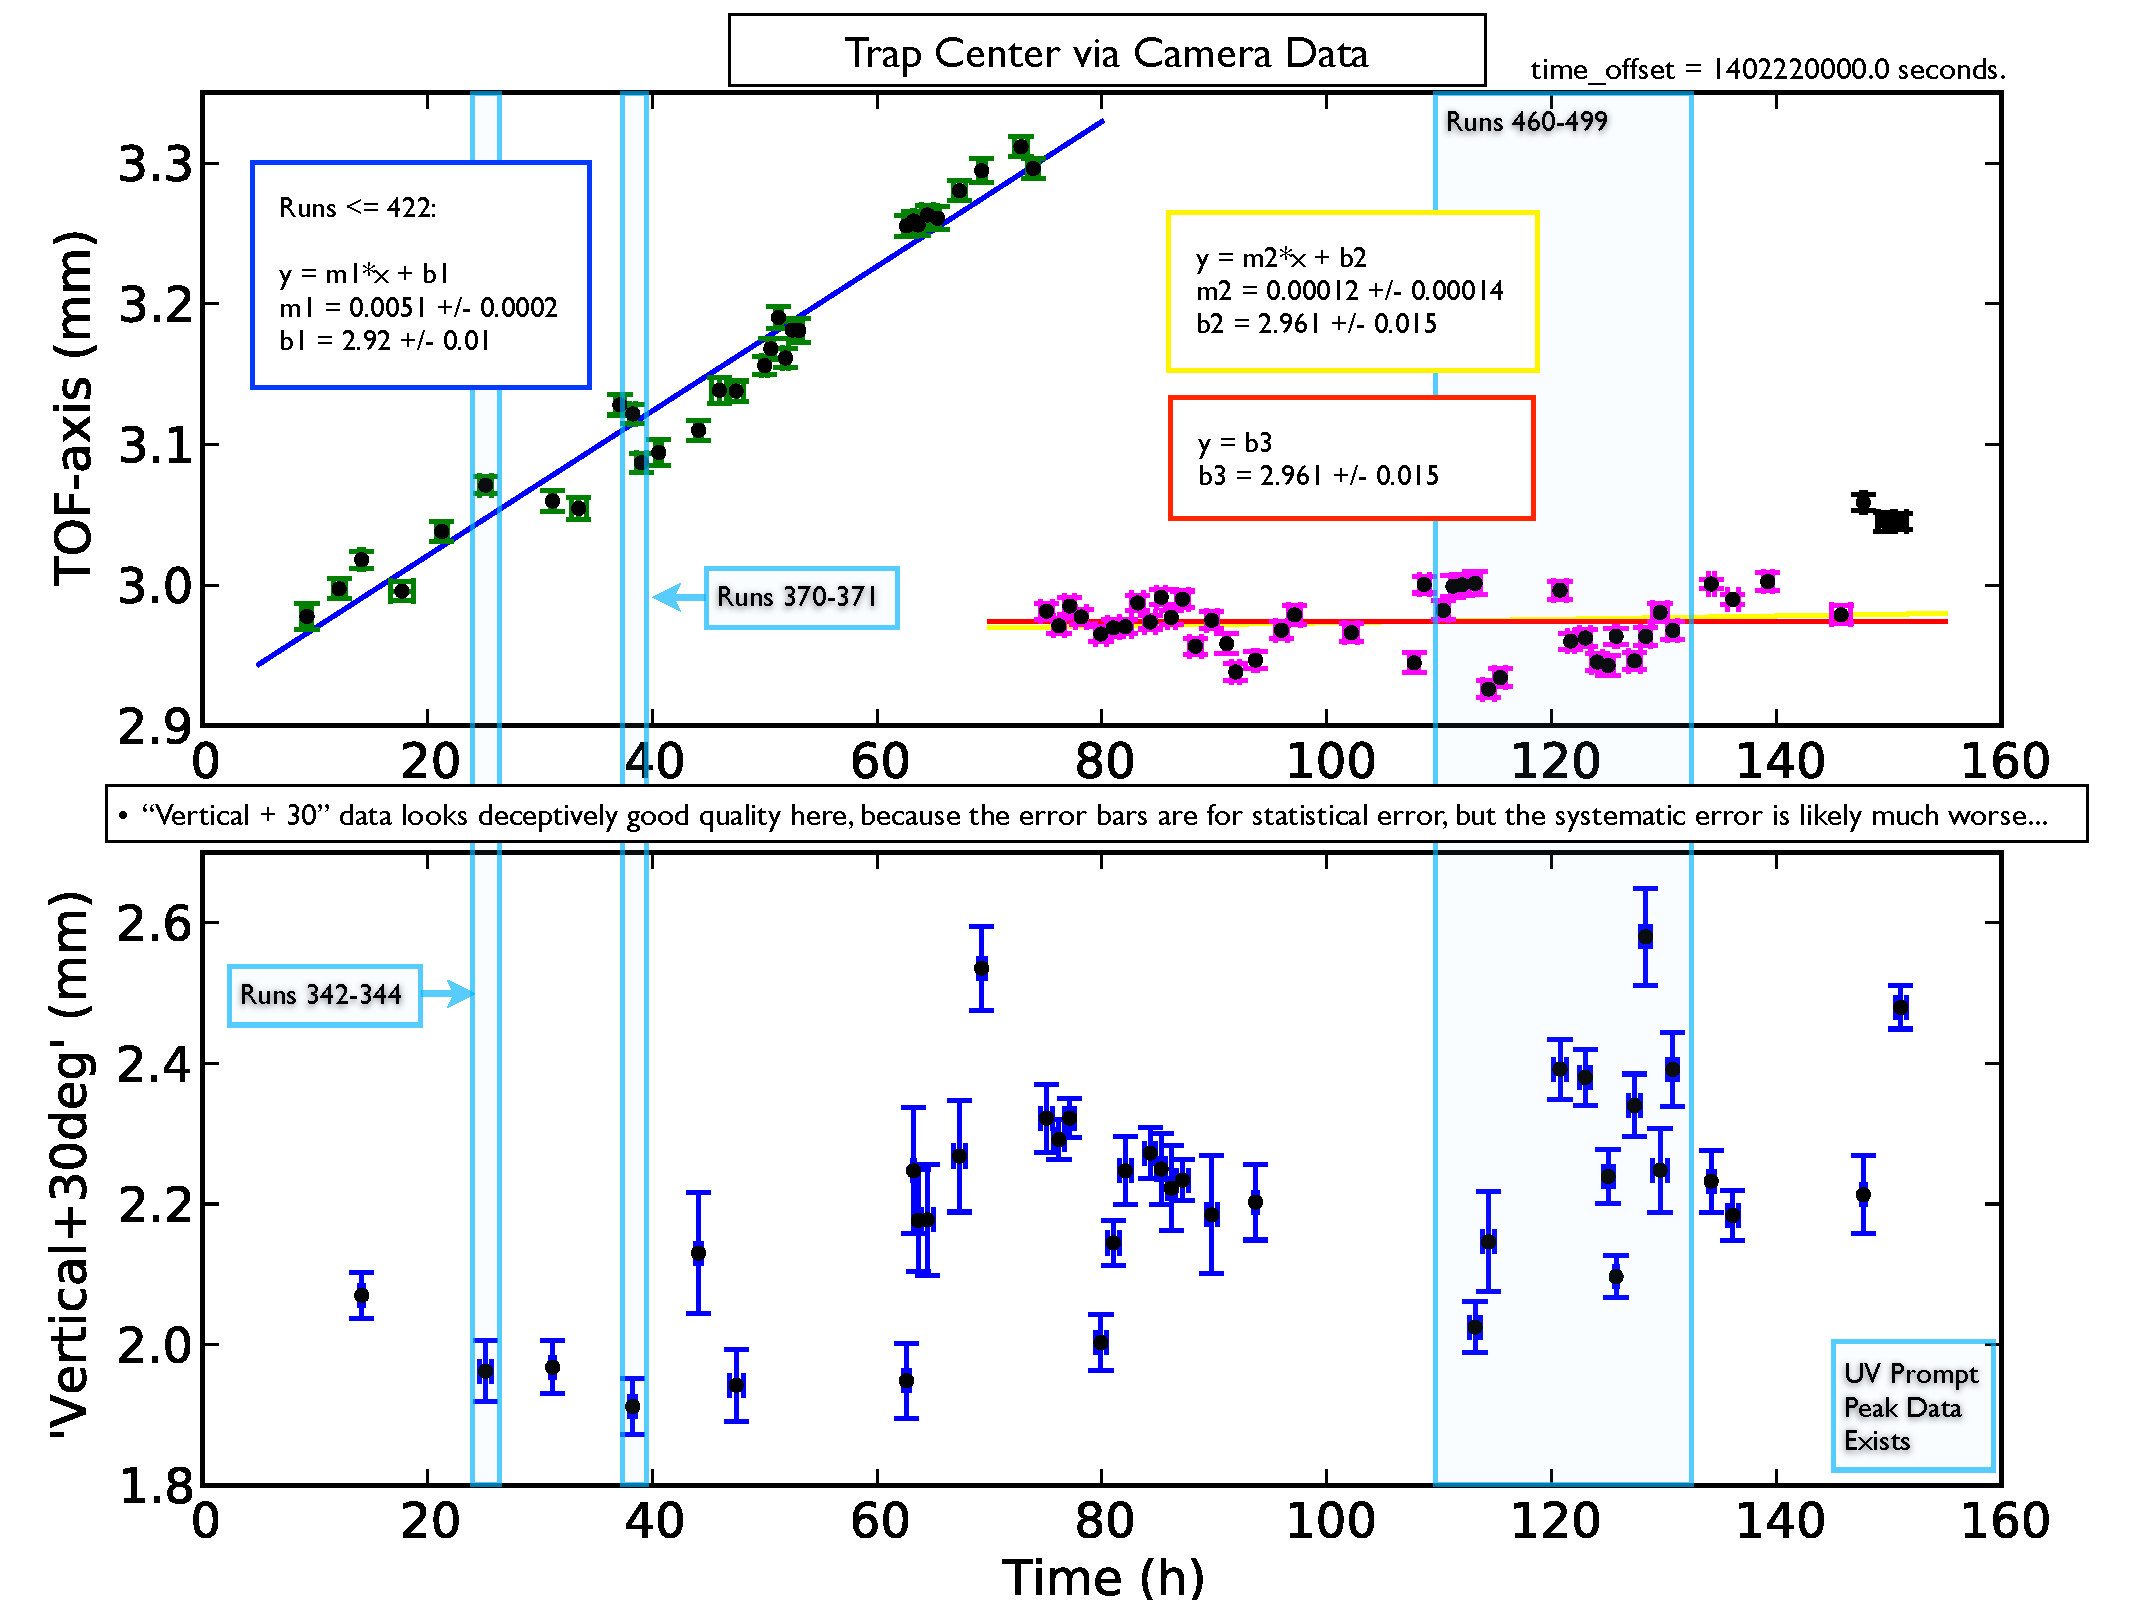
\includegraphics[width=.999\linewidth]
	{Figures/TrapPosition_FromCamera.pdf}
	\caption[Trap Position from Camera]{Trap Position along the ``Time-of-Flight'' Axis and the ``Vertical+30" Axis.  All runs plotted by time of run. \comment{(Need to re-plot this.)}}	
	\label{fig:cameraposition_by_time}
\end{figure}


\begin{figure}[h!!t]
	\centering
	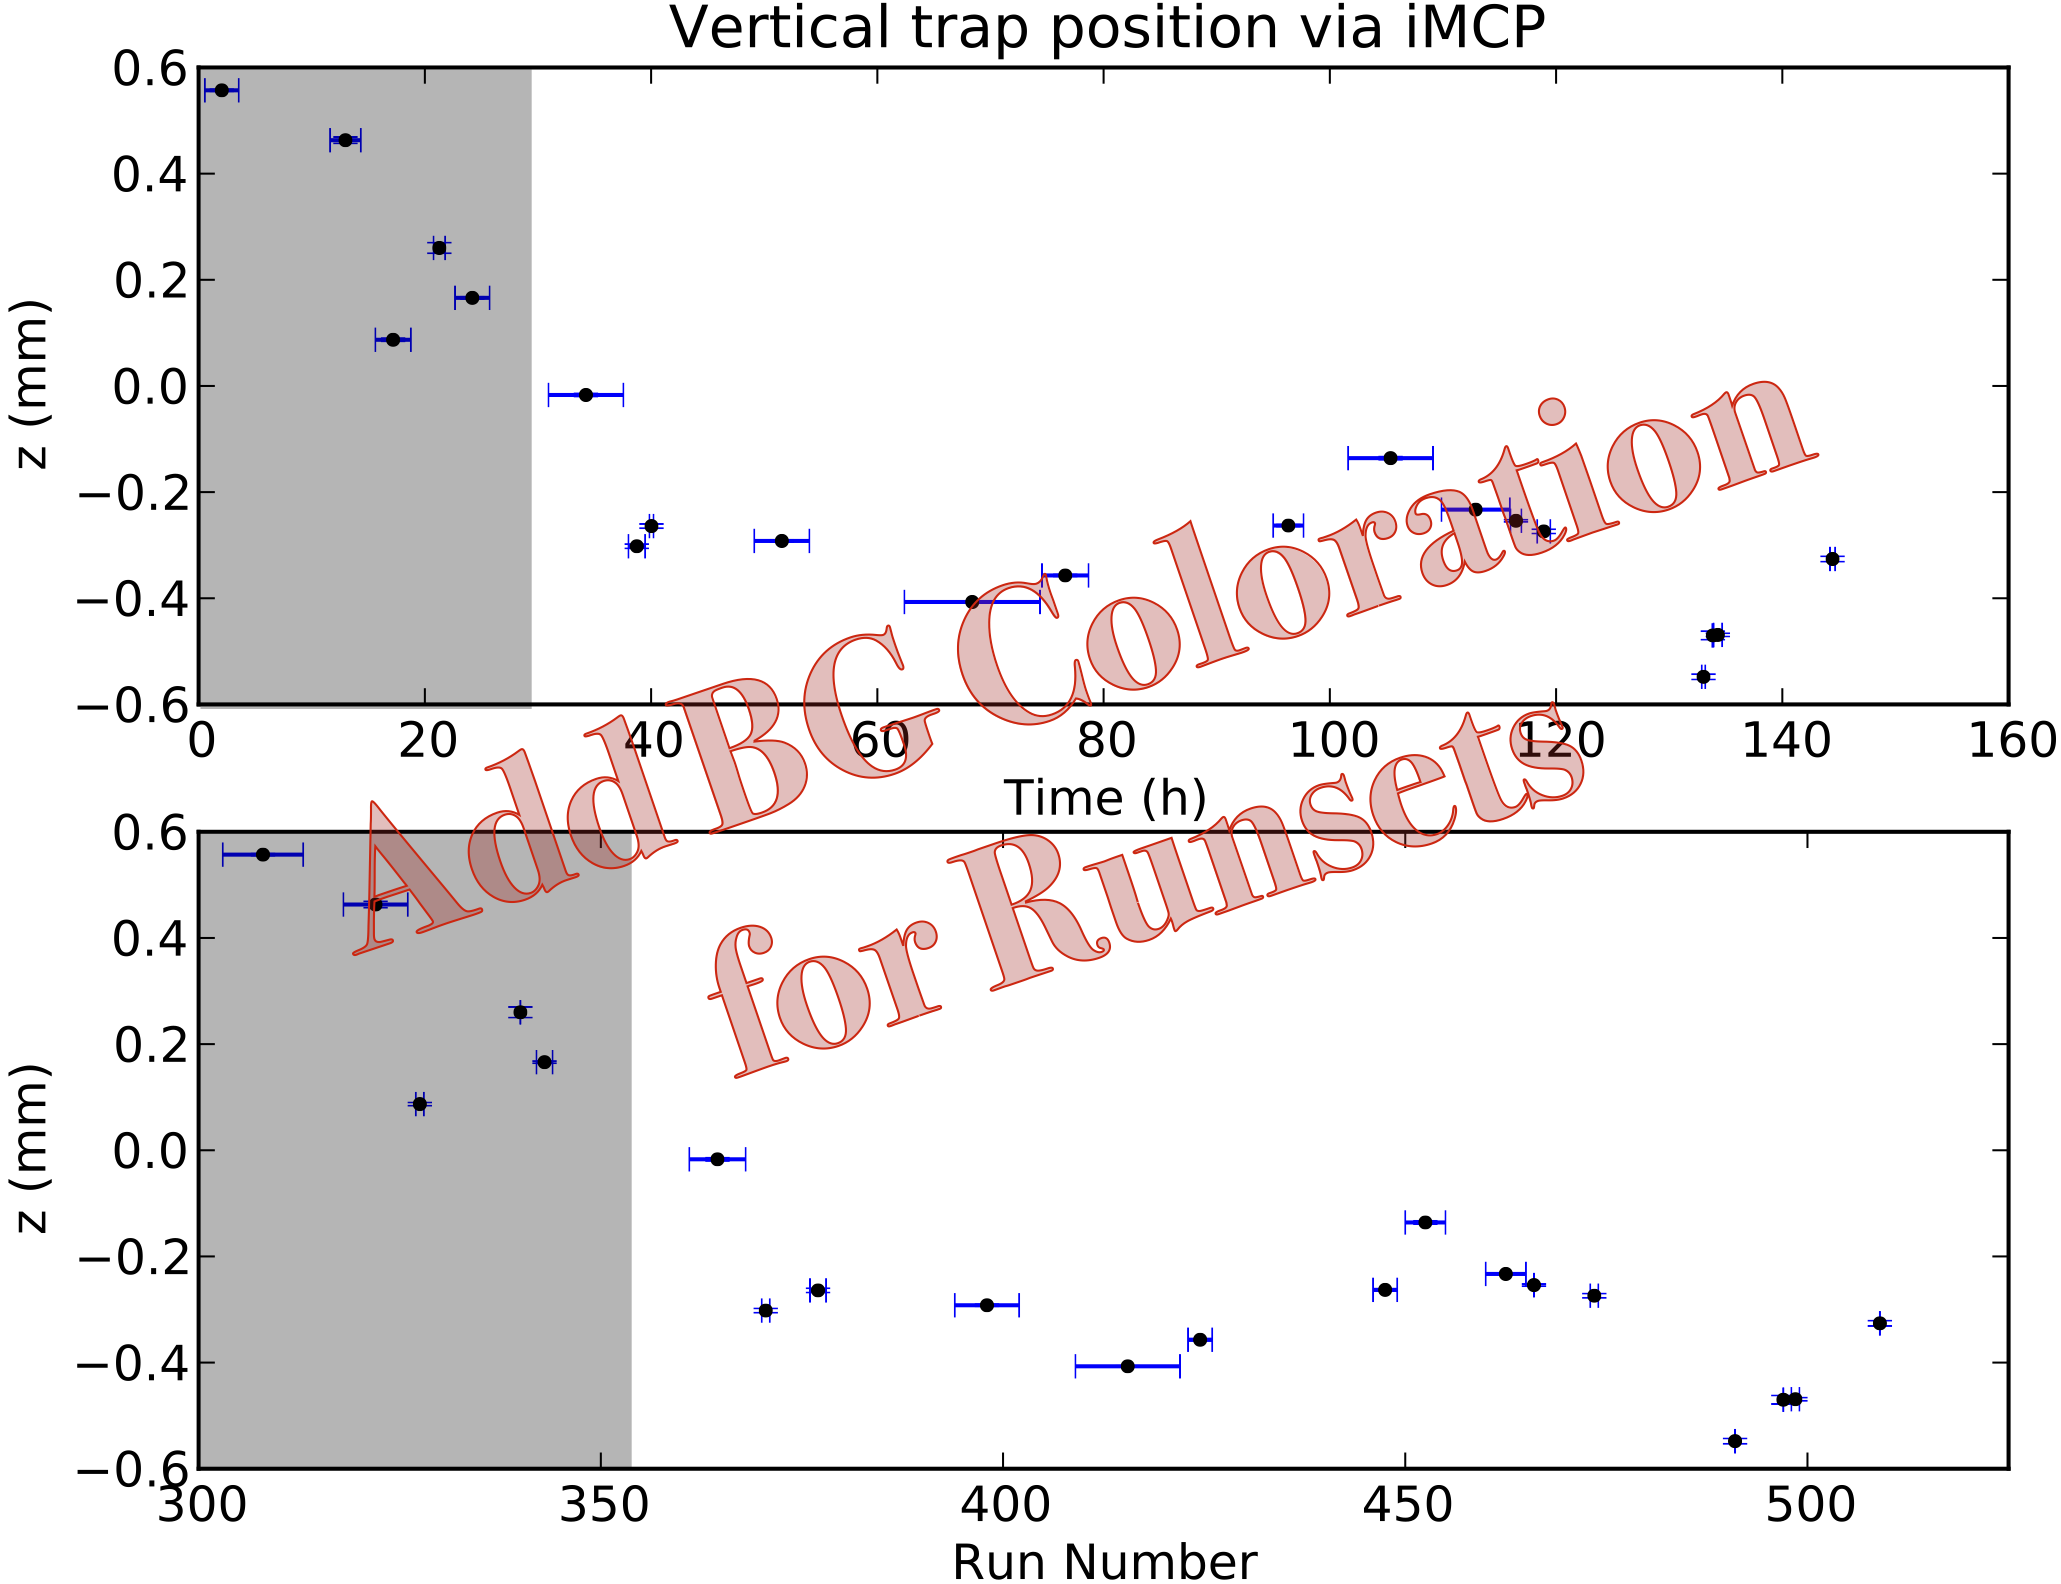
\includegraphics[width=.999\linewidth]
	{Figures/VerticalTrap_by_rMCP_prelim}
	\caption[Vertical Trap Position from rMCP]{Trap Position along the Vertical Axis, plotted as a function of time of run (top) and run number (bottom).}	
	\label{fig:vposition_by_run_rmcp}
\end{figure}


%\section{Beta Detector Cuts}
%\label{section:calibrations_betadetectors}
%	Setup is as described in Section~\ref{section:betadetectors}.	 
%	\note{This is a stupid section name.  Also, I really do need to describe how the cuts were made here somewhere, because it's non-trivial in many cases, and possibly different than what Ben did in some cases.  But it won't make sense to describe what I did different if I don't describe the thing as a whole, at least a bit.  The point is, this is a set of cuts/systematics that isn't really that straightforward to understand.  }
%\section{Plastic Scintillators}
%	\note[color=org]{Maybe this goes in Chapter~\ref{dataselection_chapter}?}
%	\note{Energy calibration for the scintillator+PMT setup changed dramatically at one point.    Describe how calibration was done.  Like, one sentence or something.  Something about the endpoint energy, and something about the compton edge for 511s, IIRC.}
%\section{Strip Detectors}
%	\note{How the fuck WERE these things done?!}



%\missingfigure{Needs an SOE timing spectrum.  At least one of them.  Experimental and simulated.  Also, I have to describe how I did the simulating, and how I check that it's OK despite the fact that the simulated spectrum looks nothing like the experimental spectrum.}


\subsection{Measurements with the eMCP}
	I can describe the eMCP calibration here, even though it mostly wasn't implemented by me.  It is tangentially relevant to data selection and background estimation by providing an experimental energy spectrum for shake-off electrons.  It's actually a pretty neat algorithm that I basically wasn't involved with.
	\note[color=jb]{JB:  eMCP.  You need to describe the timing information obtained.  You also need a statement of whether or not you used the position information in your cuts.}




%%% !TEX root = ../thesis_main.tex
%%%
%%%
%%%
%%%%%% --- * --- %%%%	
%%%%%% --- * --- %%%%	
%%%%%% --- * --- %%%%	
%%%\clearpage
%%\section{Data Selection and Preliminary Cuts Mini-Intro from John}
%%\note[color=org]{from JB, on whether to combine `Analysis' chapter with `Calibrations' chapter:  ``I see no special reason either way.  I would say the topics seem distinct.''}
%%%
%%\note[color=jb]{JB says:  ``((Ch.~\ref{dataselection_chapter})) looks fine to me.''  ...even in spite of the giant paragraph suggestions below, I guess.}
%%%\note[color=org]{Do I actually want to combine this with Chapter~\ref{calibrations_chapter}?}
%%%\note[color=org]{from JB:  you ask at the start if you should combine it (Ch.7 (now Ch.6) ((Ch.5)), `Analysis') with Ch.6 (now Ch.5) `Calibrations'. I see no special reason either way.  I would say the topics seem distinct.}
%%%\\...\\
%%%Then Section 7.1...
%%%}

%\section{Data Selection and Pre-Processing}
%\section{Run Parameters and Preliminary Cuts}
\section{Data Selection and Preliminary Cuts}
\note{We now consider how to clean up our data.  We make some fairly obvious, intuitive cuts, and those are described here.  Later, we'll make less intuitively obvious cuts.}
Although the detection chamber was designed to feature two MCP detectors on opposing sides of an applied electric field intended for simultaneous use (see Section~\ref{section:mcps}), % to collect positively charged recoiling ions on the rMCP and negatively charged shake-off electrons on the eMCP 
in practice the two detectors produced quite a bit of feedback when operated at the same time.  In order to salvage usable data from the beamtime, we ended up running only one detector at a time, but switched which detector was in use every few hours, collecting approximately the same amount of data with each detector.  Thus, the runs are sorted into `electron' and `recoil' runs, depending on what the detector in use was intended to detect.  

While the beta asymmetry and Fierz interference are best evaluated using the electron runs, the recoil runs are best for evaluating the polarization (a dominant uncertainty in the beta asymmetry measurement) and the cloud position.  The polarization measurement is the subject of a recent publication (see~\cite{ben_OP}), and the cloud position evaluation is discussed in more detail in Chapter~\ref{calibrations_chapter}.

The data is further split up into four runsets:  A, B, C, and D based on when certain detection settings were adjusted, and each of these runsets contains both electron and recoil runs.  These four runsets were then treated separately for nearly all parts of the analysis.  In particular, Data Set A was neglected completely during analysis after it was determined that one scintillator had an improperly set hardware threshold such that lower energy betas weren't being detected at all.  Additionally, there was a QDC module failure between Runsets B and C, resulting in an abrupt change in calibration for the two scintillators.  
\note{`The observant reader may find it curious that the listed runsets start at ``B'' and continue alphabetically.  There was initially a ``Runset A'' collected as well, however it was determined later that this data could not be salvaged for use in the final analysis because one of the scinitillators had its hardware threshold set above the compton peak, and without that reference point an accurate calibration could not be performed.'}

%\note{Also, the background was too noisy in Set A I think.  Also, pretty sure there isn't really that much data in Set A at all.  Also-also, Set A has E=66.7, so can't use it for more stats on the other backgrounds. ... Maybe I should just look up what the deal even was with Set A, since I don't really remember.} 

%\note{What did I change between Runsets B and C?  Between Runsets C and D?  ...OP time, yes, but also and one point a PMT(?) (eta:  it was a QDC) blew out and we replaced it, so then the scintillator calibration was a bit different afterward.  Anyway, I should maybe just make a goddamn table.  Table goes here.}

% !TEX root = ../thesis_main.tex


\begin{table}[h!!!!t]
	\begin{center}
	\begin{tabular}{ c || p{5cm} | p{5cm} | p{1.2cm} | }
			\multicolumn{1}{  c  }{ } & 
				\multicolumn{1}{  c  }{ \!\!Electron Runs\!\! } &  \multicolumn{1}{   c  }{ Recoil Runs }  &  \multicolumn{1}{   c  }{ OP Delay }  \\
			\cline{2-4}
			\multirow{1}{*}{Runset A}	& 314, 362, 363, 383, 384, 385, 386, 393, 420.
									%	& 303, 308, 309, 310, 311, 312, 313, 318, 326, 327, 328, 340, 342, 343, 361, 368, 370, 371, 376, 377, 378, 394, 395, 396, 398, 399, 400, 401, 402, 409, 410, 411, 412, 413, 414, 415, 416, 417, 418, 419.
										& 303, 308-313, 318, 326, 327, 328, 340, 342, 343, %361, 368, 370, 371, 
										376, 377, 378, 394, 395, 396, 398-402, 409-419.
										& $300\,\mu s$
										\\
			\cline{2-4}
			\multirow{1}{*}{Runset B}	& 428-437, 440-445.
										& 421-426, 446, 447, 449.
										& $300\,\mu s$
										\\
			\cline{2-4}
			\multirow{1}{*}{Runset C}	& 476, 477.
										& 450, 454, 455, 460-466, 473, 474.
										& $700\,\mu s$
										\\
			\cline{2-4}
			\multirow{1}{*}{Runset D}	& 478-489, 502, 503, 504, 505, 510, 513.
										& 491, 497, 498, 499, 509.   
										& $400\,\mu s$
										\\
			\cline{2-4}
	\end{tabular}
	\end{center}
	\note{MUST check to make sure I didn't use Run 420 in ``good runs" in the end!!!}
	\note{I have more (really early) runs classed in Set A than Ben had.  In the end, we didn't use them so it doesn't matter.  But...what?}
	\note{Ugh.  My categorization system is slightly different than Ben's on the later recoils.  That's annoying.}
	\note{Other things I could list here:  Electric field strengths, total runtime.}
	\caption[List of Runs]{A list of 2014 online runs with potentially usable data.  Runset A was discarded completely due to problems with hardware threshold settings.  There was a QDC module failure before Run 450, so it and all subsequent runs were performed using a different module, and as a result the scintillator calibrations changed slightly at this time.  Anyway, the point of this thing is to show which electron runs and recoil runs go together, for the purposes of evaluating polarization and cloud attributes.}
	\label{table:runlist}
\end{table}


% !TEX root = ../thesis_main.tex


\begin{table}[h!!!!tb]
	\begin{center}
	\begin{tabular}{ c || p{1.2cm} | r | l | p{5.8cm} | }
		\multicolumn{4}{l}{Electron Runs} %& \multicolumn{1}{l}{Electron Runs} 
		\\
		\cline{1-3}
		\multicolumn{5}{c}{ }
		\\
			\multicolumn{1}{  c  }{ } & 
				\multicolumn{1}{  c  } { \!\!OP Delay\!\! } &  \multicolumn{1}{ c }{ \!\!Events\!\! }  
				& \multicolumn{1}{ c }{ \!\!Electric Field\!\! } & \multicolumn{1}{ c }{ Runs } 
				\\
			\cline{2-5}
			\multirow{1}{*}{Runset A}	& $300\,\mu s$
										& 0
										& \,\,\,$66.67$ V/cm
										& 314, 362, 363, 383-386, 393. %, 420.
										\\
			\cline{2-5}
			\multirow{1}{*}{Runset B}	& $300\,\mu s$
										& 173,640
										& $150.0$\,\, V/cm
										& 428-437, 440-445.
										\\
			\cline{2-5}
			\multirow{1}{*}{Runset C}	& $700\,\mu s$
										& 18,129
										& $150.0$\,\, V/cm
										& 476, 477.
										\\
			\cline{2-5}
			\multirow{1}{*}{Runset D}	& $400\,\mu s$
										& 207,596
										& $150.0$\,\, V/cm
										& 478-489, 502-505, 510, 513.
										\\
			\cline{2-5}
	\end{tabular}
	\end{center}
	\note{A list of 2014 online runs with potentially usable data.  Runset A was discarded completely due to problems with hardware threshold settings.  There was a QDC module failure before Run 450, so it and all subsequent runs were performed using a different module, and as a result the scintillator calibrations changed slightly at this time.  Anyway, the point of this thing is to show which electron runs and recoil runs go together, for the purposes of evaluating polarization and cloud attributes.}
	\note{Ben doesn't seem to include Runs 436 and 437 in *any* set of good runs.  Is it an oversight?  I think they're perfectly legit electron runs.  They're fairly long runs...}
	\caption[List of Electron Runs]{A list of electron runs and associated parameters.  The ``Events'' column includes only the number of events that passed all cuts.}
%	\note{This table might eventually go away.  Mostly I just want a record of the total `good' counts.  In total, $N=399,365$.}
	\label{table:runlist_electrons}
\end{table}



Before proceeding further, several basic cuts are performed on the data.  For the Electron Runs which are to be processed directly into a physical measurement, we consider only events in which there was a recorded hit \emph{both} on the eMCP \emph{and} on (at least) one of the scintillators.  The required scintillator hit, of course, is potentially a beta, and so it is obvious why this must be present.  The eMCP hit requirement -- particularly with the timing of the eMCP hit occuring within a certain time range relative to the scintillator hit -- is used to tag beta decay events originating from the cloud, as opposed to those originating from some other surface within the chamber.  The precise time interval to be used, and how its results should be evaluated,\aside{also discussed: how we decide what counts as an eMCP hit at all} is discussed in Section~\ref{section:emcp_cuts}, but for the first pass through the data it is good enough to simply require that an eMCP hit occurred.\aside{Awkward stupid phrasing.}  Although not every beta decay event from the cloud will produce a hit on the eMCP, this requirement eliminates a great deal of background that would otherwise be challenging to evaluate.  \aside{Also, we claim that it doesn't bias the data.  Much.  Didn't I try to evaluate how much it biased the data at one point?}  
 
%The scintillator hit is considered to be potentially a beta from a decay
Because the eMCP hit is required as a `tag' of good events, it is also necessary to remove from direct consideration any event which is coincident with a pulse of the photoionization laser.  When photoionization occurs within the atom cloud, an orbital electron is removed from the atom and will be accelerated by the electric field into the eMCP, just as a shake-off electron from a decay might be.  If, by chance, this photoelectron arrives in coincidence with a scintillator hit, it would be interpreted as a decay event from the trap -- unless we preemtively discard it.  


Over the course of the runtime, there were several instances where we noted an apparent electrical discharge within the experimental chamber, producing enormous backgrounds for a short time.  The detectors typically recovered quickly afterward, so it was neither necessary nor useful to stop an entire run to wait for the system to recover.  Instead, the time when the discharge occurred was recorded, and events within approximately one minute of the spark time were discarded.  

%Because it is of the utmost importance to understand the nuclear spin-polarization immediately prior to a decay, 
We use only the ``fully polarized'' events for which we have a detailed understanding of the nuclear polarization (described in more detail in ~\cite{ben_OP}).  This means we must use \emph{only} events from the ``optical pumping'' portion of the duty cycle (see Fig.~\ref{fig:dutycycle}), and discard events when the DC- or AC-MOT is active.  After the AC-MOT is shut off, there is a short delay before optical pumping begins (see Table~\ref{table:runlist}) to allow the magnetic field to decay, and it is only after $100\,\mu s$ of optical pumping that we consider the atoms to be fully polarized.  Furthermore, because the magnetic field from the DC-MOT is slow to decay (relative to the field from the AC-MOT), all events from the first five AC/OP cycles after every atom transfer are discarded.  A secondary benefit of our insistence on considering only polarized data is that the scintillators' gains are more stable in the presence of only the (small, stable) magnetic field used for optical pumping than they are in the presence of a larger oscillating magnetic field used for trapping.
\note{change by 0.2\% of its value vs change by 0.5\% of its value, according to Ben's thesis pg 143.}

%Another class of event that must be removed from direct analysis is 
Finally, because this analysis depends heavily on energy measurements from the two scintillators as a proxy for beta energy, it is necessary to remove events in which the pulser LED fired.  Although the pulser LED is useful for evaluating the stability of the scintillators, in the case where an LED pulse occurs together with a true beta hit in the scintillator, it may change the measured energy.  Therefore, we discard all events that include an LED pulse.   
	

\section{Further Cuts Using the DSSD}
%\note[color=org]{Have I even defined `DSSD' yet?}
\note[color=org]{Pretty sure I'm repeating myself from Chapter~\ref{???}}
\note[color=jb]{JB says: To repeat a comment, since the Appendix on analysis changes is being dispersed throughout, when you state somewhere (I think it's in Ch. 6)((5?)) make sure you state clearly that the only change for BB1 cuts
is the radius cut, e.g. that you took the same T and E from the waveforms (I'm not even sure whether the
waveforms are recorded anyway). You  ask 'how can I state this' but there's no reason to be subtle.
Just say upfront that Ben and Spencer's theses did all the groundwork on the BB1, and here you include selected details needed to understand the present analysis. If you need to include some redundant material, don't worry too much about that.
\\ ... \\ 
MJA:  In fact, I think the BB1 radius may have been the same.  The uniform energy threshold was different though.  But I get the point.
\\ ... \\ 
Also, yes, the waveforms are absolutely recorded in the MIDAS files but they haven't been saved to modern ntuples, because they made the files huge.  I think it's probably pretty easy to switch that on/off in the Analyzer though to generate a set of ntuples that has that info included.
}

\missingfigure{Show individual beta energy spectra.  ...with a variety of different cuts, perhaps?}


Although it was not possible to use the DSSD in real-time analysis or event triggering, the DSSDs may be used, after the data has been collected, to distinguish between different types of particles incident on the detector, as more energy will be deposited by heavier particles.  When a scintillator hit is triggered by a particle originating within the experimental chamber, that particle will typically have passed through the DSSD before arriving at the scintillator.

In the present experiment, the two primary particles that will concern us are $\beta^+$ particles originating from the decay of $\isotope[37]{K}$, and $\gamma$ rays, which may be produced through a variety of processes, e.g. directly from the $2\%$ decay branch, through annihilation of $\beta^+$ particles upon their interaction with regular-matter electrons, or bremsstrahlung radiation from emitted $\beta$s.  

We would like to look specifically at events involving $\beta^+$ particles arriving direct from a decay within the atom cloud, and the DSSD may be used to eliminate events in which the scintillator is triggered by a $\gamma$.  An incident $\beta$ will typically deposit some portion of its energy in the DSSD as it passes through, however an incident $\gamma$ will deposit significantly less energy; for this setup the energy deposited by a $\gamma$ is generally indistinguishable from background on the DSSDs.  Therefore, we require that a `good' event must include a `good' hit to the DSSD as well as a hit to the associated scintillator.   

In order to proceed at this point, and because the DSSD readout records so much information, it is necessary to develop some criteria to determine whether or not we will accept any given DSSD readout as a $\beta$ hit.

\note{How do I *say* that Ben was the one who did most of the DSSD calibration stuff?  I maybe don't need to describe all of it here, but I *could*, and maybe it's needed in order to understand like 4 rows in my error budget.}  

\note[color=jb]{JB:  ``You can describe anything you did differently or improved, but you can and should otherwise defer all details of the scintillator calibration and DSSD calibration to Ben's paper and his thesis and Spencer's.  E.g. Section~\ref{section:bb1_systematics} ``statistical agreement between BB1 X and Y detectors' energies only makes a small effect on results" does not need the technical details beyond that statement.''
\label{thesisconventionjb} }
\note[color=jb]{JB:  ``If you have some way of documenting the coding you used, that would be great.''  ... yeah, it would, wouldn't it?}


We read out the full waveform for every strip at each event with a scintillator hit, but in post-processing take \emph{only} the `time' and `energy' from the peak waveform height and the time in the waveform at which that occurs. Each strip will have its own noise spectrum and energy calibration.  To classify an event as a good DSSD hit, we require at least one `x' strip and one `y' strip record an energy above the noise threshold.  We require that the x strip and the y strip agree (to within some number of standard deviations) in amount of energy deposited, and in the time at which that hit occurred.  In order to avoid problems resulting from the strips' non-uniform noise thresholds, we further require that the energy deposited be greater than some lower-end cutoff which is selected so as to be higher than every individual strip's noise threshold.  In this case, the DSSD's lower energy uniform threshold was set at 50 keV.  

\note{I think Ben might have selected 60 keV?  That's maybe something for the appendix.}

We also elect to use only events where a beta hit the DSSD within a $15.5\,$mm radius of the center of the detector, so as to avoid scattering effects from the collimator walls. \aside{Did I even mention the collimator?  Like, in the previous chapter or something..?}

%Look at all the events to determine how noisy each individual strip is.  Do that for all strips.  Is the energy higher than some noise threshold?  by like a few sigma?
\note{Also-also (did I mention it already?) look for events with only *one* DSSD hit (two could indicate the beta scattered back out of the detector in another pixel, or alternately an accidental coincidence of two beta decay events.  either way, no good for analysis.)  Also, only one scint hit, and it has to be the on the same detector with the DSSD.   (...A scintillator hit as indicated by a TDC readout, as well as a max. recorded scint energy for the ``extra'' scintillator at something stupidly tiny, like 10 keV.  Probably *actually* 10 keV.) }

\note{After all other cuts -- not before!! -- we eventually use only events with scint energy between 400 - 4800 keV.  High cutoff is because of the low number of events, which makes the observable--the superratio asymmetry--poorly defined and poorly behaved.  Low cutoff is because it's really hard to model what's going on down there to the required level of precision.  The observable depends most heavily on low beta energy events, so it is imperative that the lower energy portion of the spectra be thoroughly understood if they are to be used for analysis. }
\note{Somewhere I should list what the energy cutoff is for this spectrum.  Or semi-equivalently, the Q-value.}

\section{Further Cuts Using the eMCP}
\label{section:emcp_cuts}
\note[color=org]{I described the HEX-75 somewhere in a previous chapter, right??}

The eMCP features a set of three delay lines, intended to be used to record the position of a hit, as in Fig.~\ref{fig:emcp_position}.  \aside{Do I need to describe MCPs and delay lines somewhere?  Maybe not...}  Though only two delay lines is sufficient to determine the position within the plane of the MCP if they are both hit, the presence of a third delay line allows for some redundancy.  In practice, however, a large fraction of otherwise `good' events include a hit on the eMCP, but have insufficient information recorded on the delay line channels to reconstruct a position.  

\begin{figure}[h!!!!t!]
	\centering
	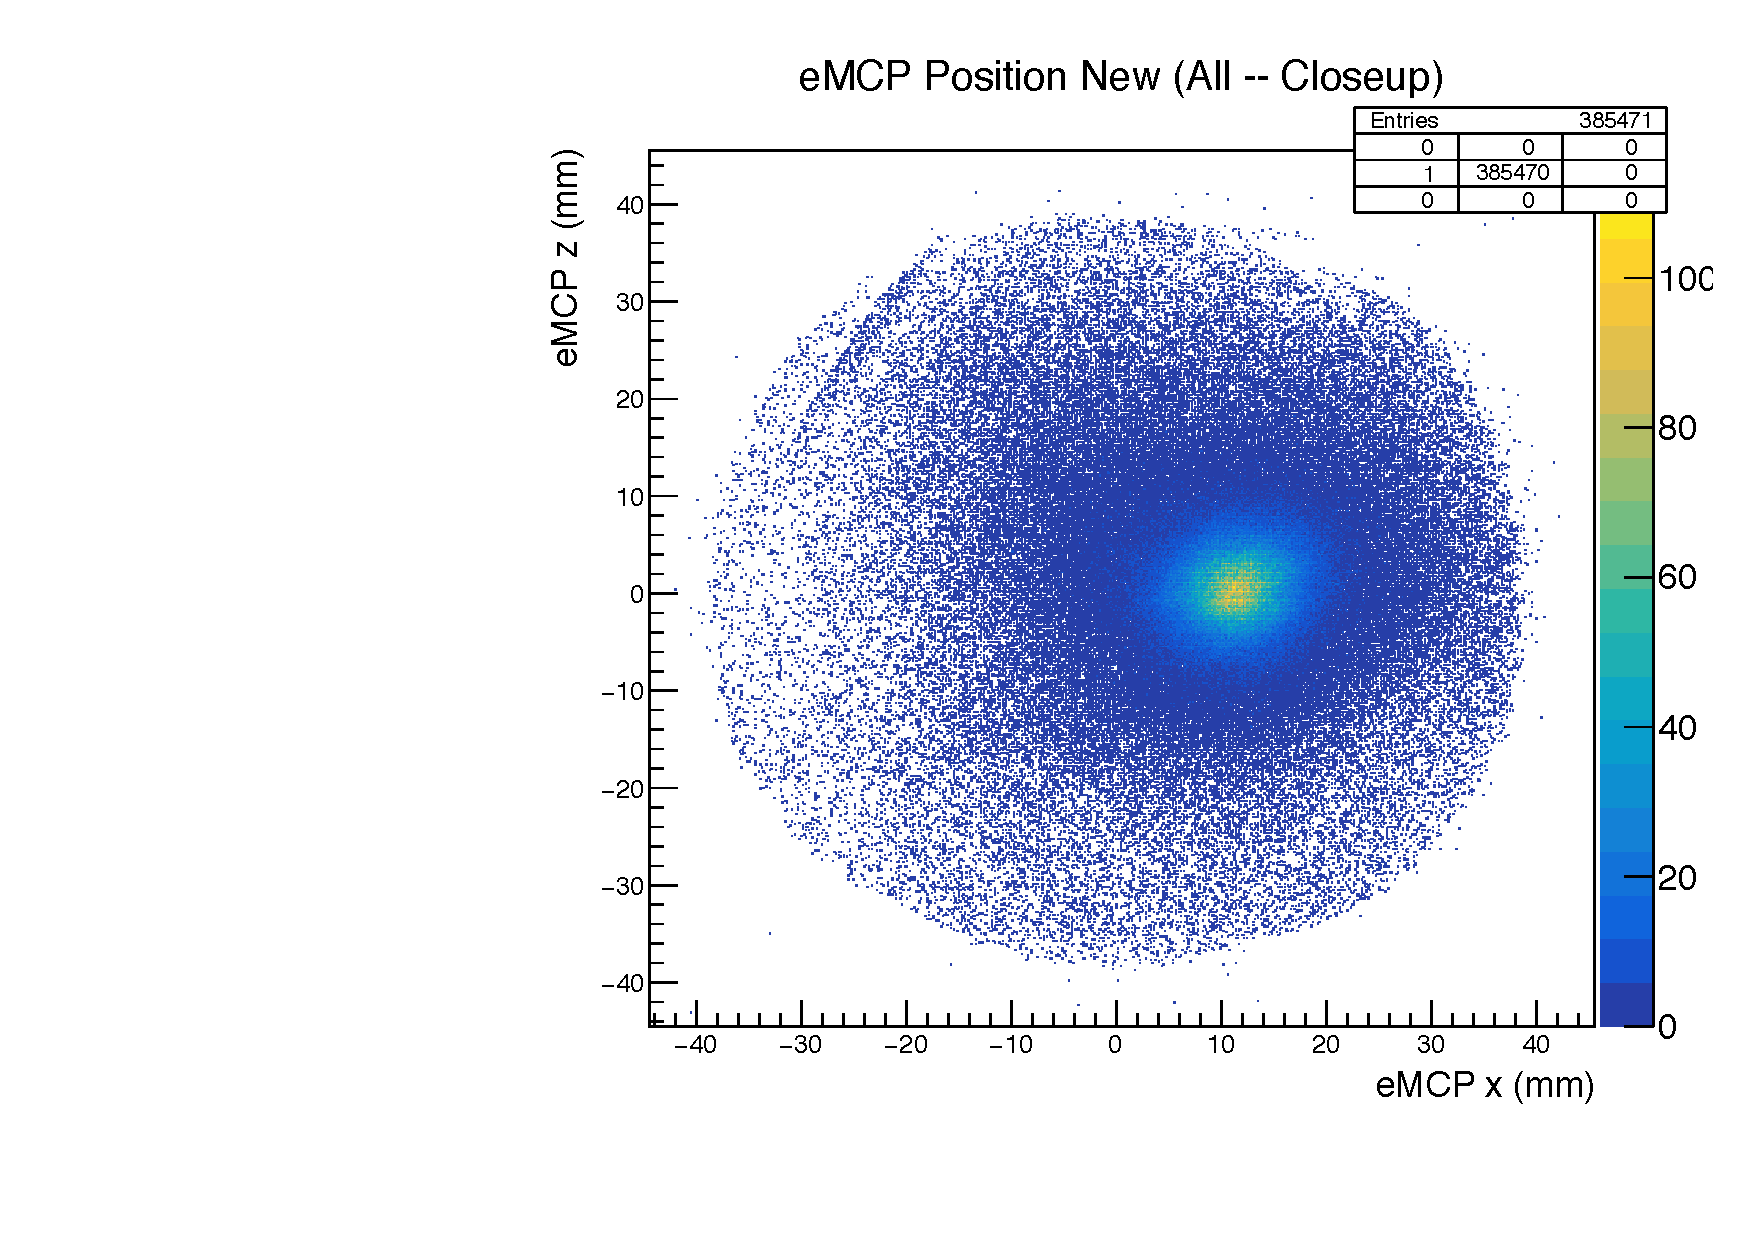
\includegraphics[width=.999\linewidth]
	{Figures/eMCP_position.pdf}
	\note{This picture is `slow'.  Need to re-save it as a png.}
	\caption{Position as measured on the eMCP, after some data cleaning.}	
	\label{fig:emcp_position}
\end{figure}

Because a SOE from the trap is most likely to land in the centre of the plate, while the background from other sources is roughly constant across the plate, it might make sense to accept only events where the eMCP hit is within some radius of the central peak.  This methodology was seriously considered because the remaining data has a much lower fraction of background events polluting it -- however this results in a loss of around half of the events even for the most generous eMCP radius cuts (see Fig.~\ref{fig:soe_tof_positioncompare}).  Therefore, it was decided that no position cuts on the eMCP would be made in the final analysis.

\begin{figure}[h!!!!t!]
	\centering
	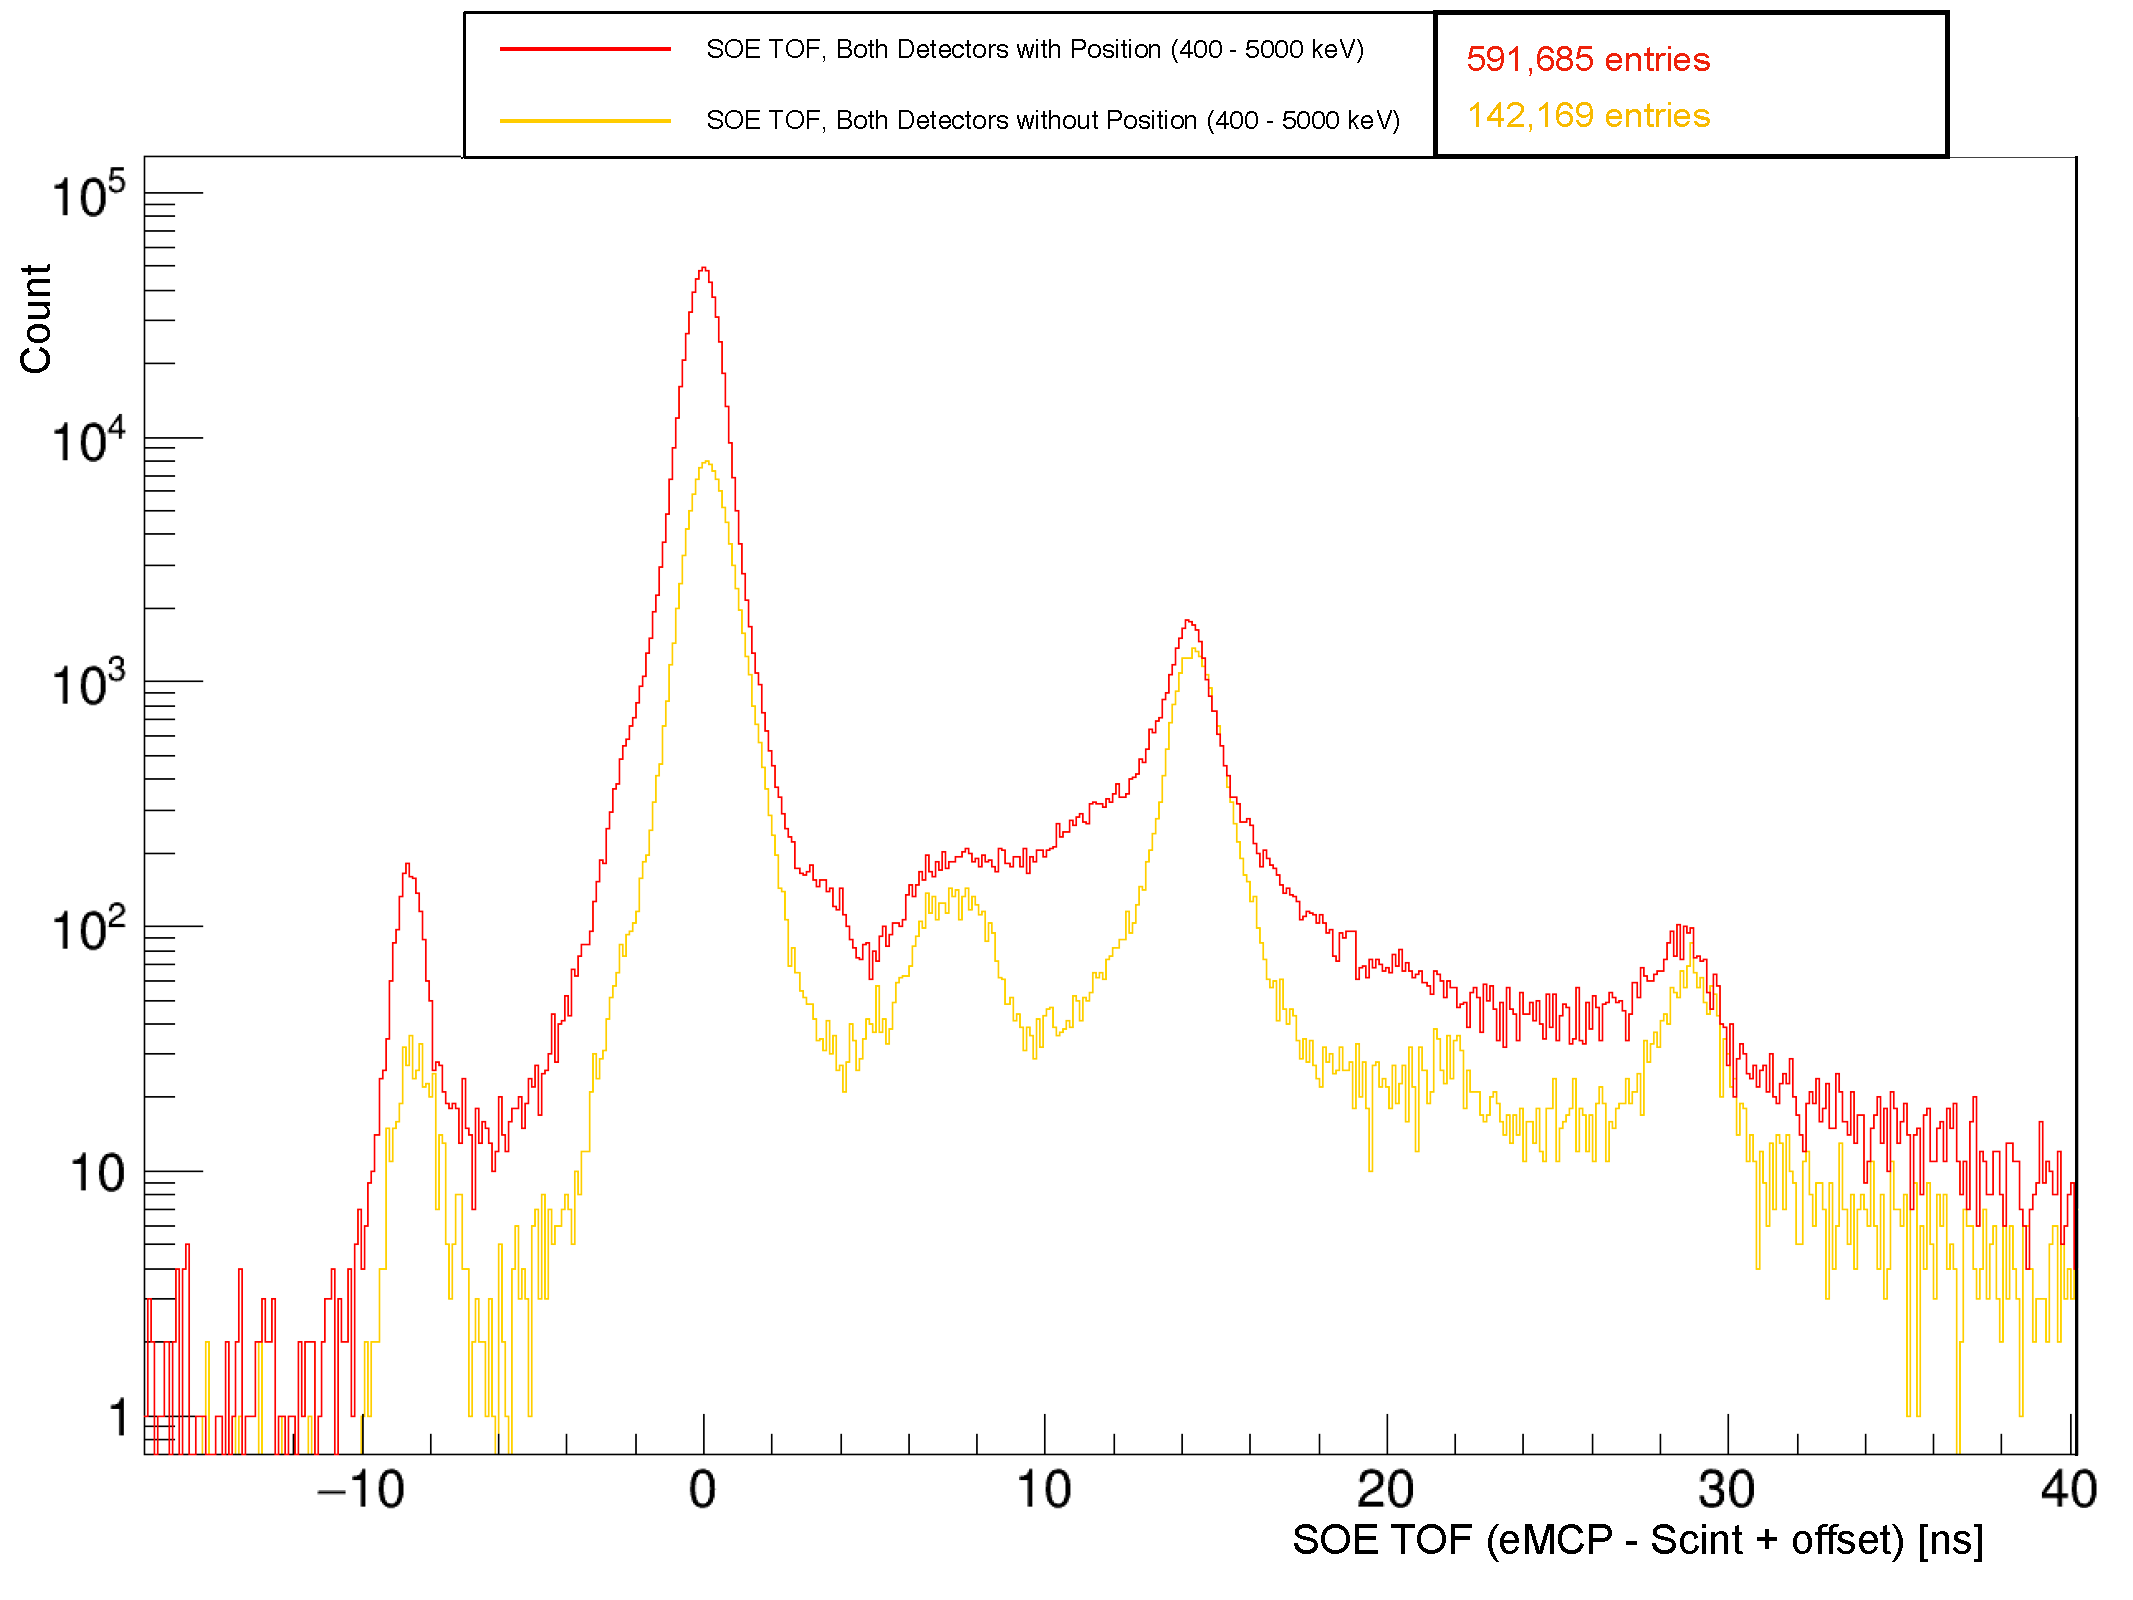
\includegraphics[width=.999\linewidth]
	{Figures/SOE_TOF_positioncompare.pdf}
	\note{Um.  Did I for sure get the labels correct on this???  It seems really wrong.}
	\caption{Beta-electron TOF, for events with and without eMCP hit position information.  A cut will eventually be taken to accept only events sufficiently near the largest peak -- in this case the number of events is `only' decreased by a factor of 2.}	
	\label{fig:soe_tof_positioncompare}
\end{figure}

Several years after the data was initially collected, a problem was discovered with our low-level analyzer software, which we had been using to convert large and unwieldy MIDAS data sets into somewhat smaller and more manageable ROOT data sets.  In particular, for every timestamp recorded, our raw MIDAS data actually included both a timestamp for the leading edge (LE) of the pulse, and a timestamp for the trailing edge (TE).  The analyzer had--for years--been reporting the timestamp associated with the trailing edge of the pulse.  Initially it was unclear if there might have been a reason behind this choice, but a closer examination of the data showed that the LE data included less timing jitter and noise, as well as a sharper peak for timing pulses across the board (as in Fig.~\ref{fig:LE_TE}), with some channels showing a larger effect than others.  This was corrected, and the entirety of this analysis has been performed now using the cleaner LE spectra.  

\note{The LE spectra allows for us to use a more precise model of the SOE TOFs, so that's nice.}

\begin{figure}[h!!t!]
	\centering
	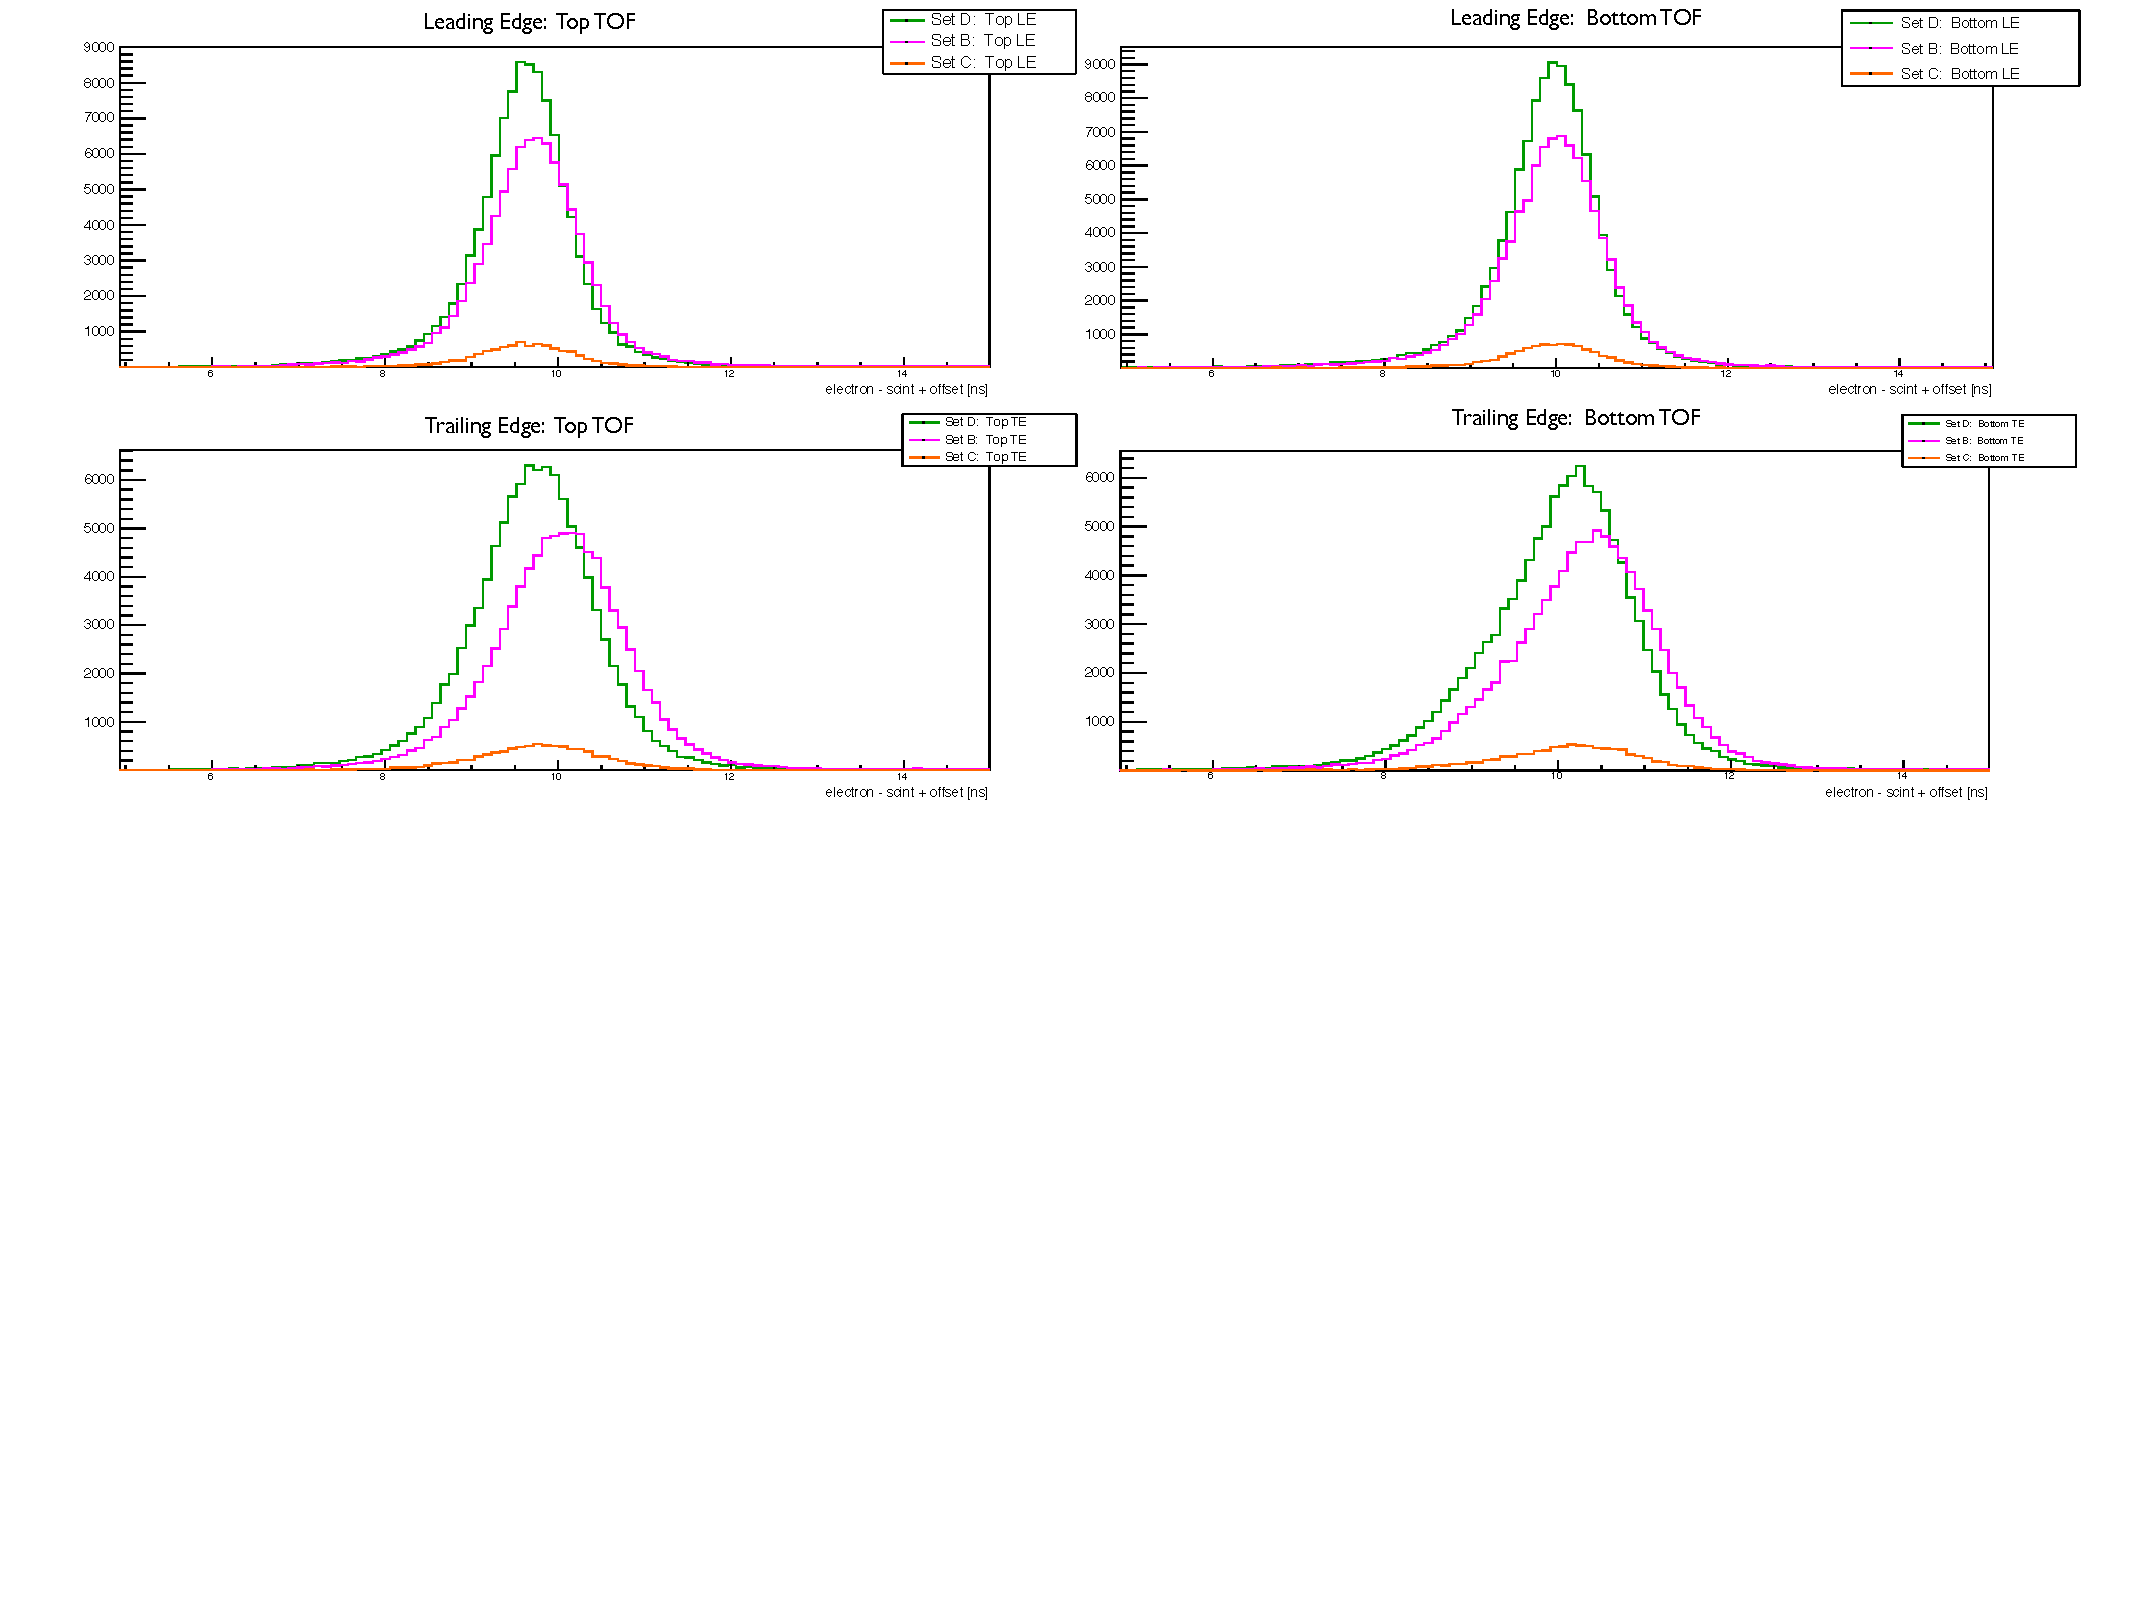
\includegraphics[width=.999\linewidth]
	{Figures/LE_TE_peaks.pdf}
	\caption{SOE TOF peaks (eMPC - Scintillator), using the leading edge (LE) and using the trailing edge (TE).  Data is sorted according to runset.  For each individual runset, the TE peak is broader than the LE peak.  The centroid of each runset is also more variable in the TE plots.}	
	\label{fig:LE_TE}
\end{figure}

The place where this change between the TE and LE timestamps had the biggest impact on the analysis is in the shake-off electron time-of-flight spectra, on which a cut must eventually be taken. Although this problem was not discovered in time to be used in the previous measurement of $\Abeta$ using this same data~\cite{ben_Abeta}, it likely would have had a negligible effect on the final result, because the SOE TOF cut that was used there was comparatively loose, and the evaluation of the background that remained was not a dominant systematic effect. \aside[color=org]{This goes in that one appendix, if I haven't already put it there.}

With the data reprocessed using the leading edge for timestamps, I wanted to eliminate as much background as possible from the SOE TOF spectrum.  With this goal in mind, the next step was to correct the scintillator timing for its low energy `walk' (see Fig.~\ref{fig:WalkAdjust}).  A quartic polynomial was fit to each of the 2D timing vs energy spectra (the top and bottom detectors were treated separately), and the result was used to produce a `straightened' SOE TOF spectrum with respect to measured scintillator energy, and as expected, the resulting SOE TOF spectrum was a bit more sharply peaked.  


\begin{figure}[h!!!!tb]
	\centering
	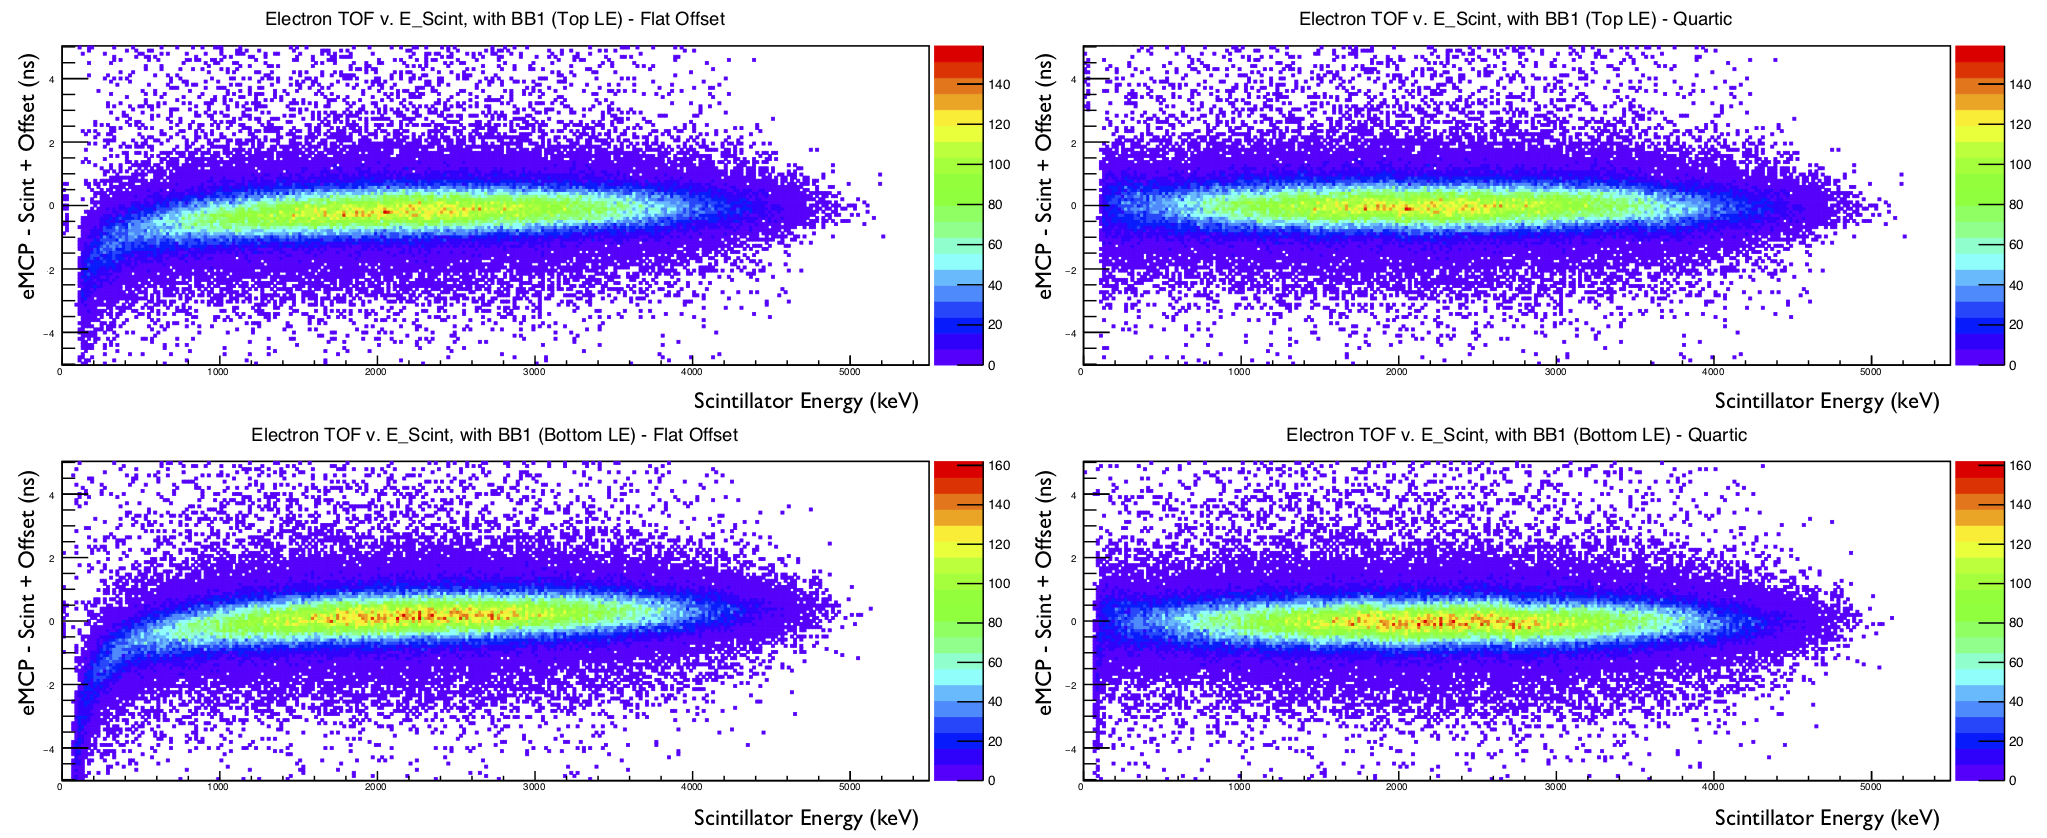
\includegraphics[width=.999\linewidth]
	{Figures/WalkAdjust.png}
	\caption{SOE TOF walk, before (left) and after (right) applying a quartic adjustment to straighten out the effective TOF.}	
	\label{fig:WalkAdjust}
\end{figure}

%At this point it becomes necessary to attempt to model the SOE TOF spectrum, as in Fig.~\ref{fig:soetof}.  
With the SOE TOF spectra cleaned up, a cut can be taken to reduce the fraction of background events.  Informed by the model of background spectra described in Section~\ref{sec:tof_bg}, a was made to include only a 2.344 ns window around the primary peak in further analysis \aside{``...removing X fraction of the remaining events."}. (see Fig.~\ref{fig:soetof}).
\note{Probably need to put that figure somewhere else.}

%For this analysis, the decision was made to use only events within a 2.344 ns window around the primary peak (Fig.~\ref{fig:soetof})  
%This part
%To understand the events that remain after this cut, it is necessary to create a model of the background events represented therein.   This is discussed in Section~\ref{sec:tof_bg}.

\note{``To check the agreement of the model with reality, we compare the averaged superratio asymmetries from both, as in Fig.~\ref{fig:asymmetry_by_tof}.'' .... probably goes in the other section.}
%\note{Okay.  This needs more description.}

\begin{figure}[h!!!!tb]
	\centering
	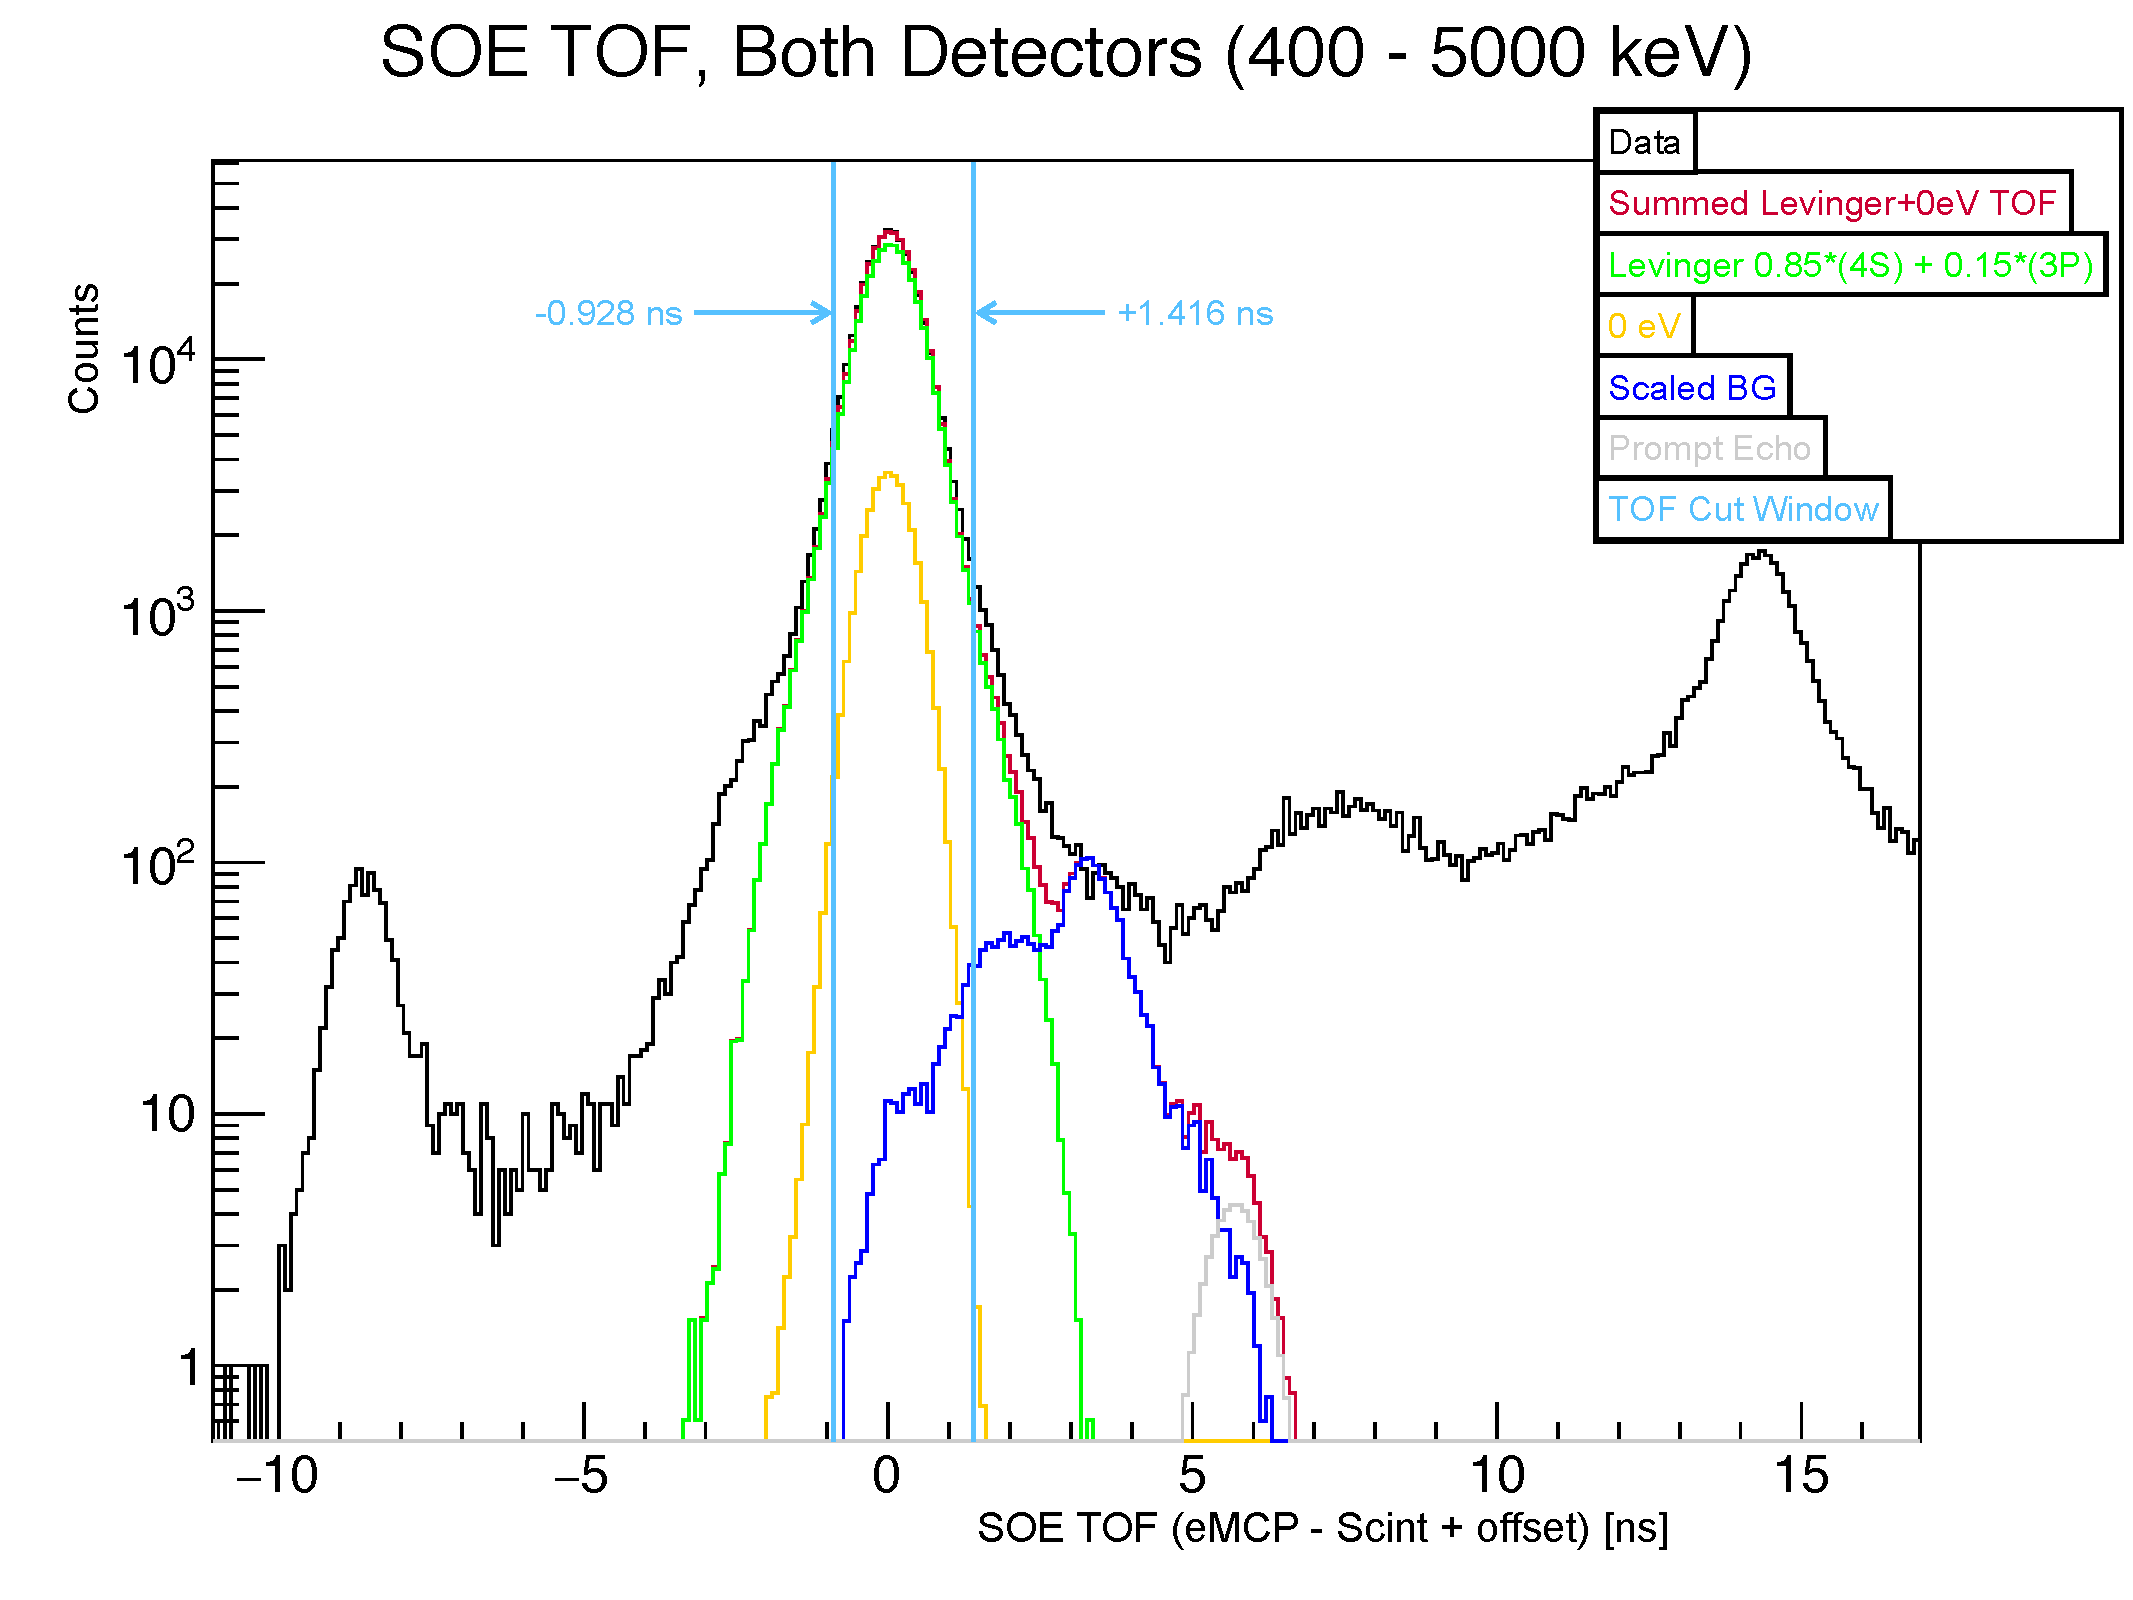
\includegraphics[width=.999\linewidth]
	{Figures/SOE_TOF_Spectra.pdf}
	\caption{SOE TOF, model and data.  In the end, I cut the data to use only events with a TOF between -0.928 ns and +1.416 ns.  Max. possible background is like a factor of two too big.  Similar quality results no matter how you distribute the Levinger spectra between 4S and 3P, however adding the 0 eV electrons makes a big improvement to the agreement. }	
	\label{fig:soetof}
\end{figure}

\begin{figure}[h!!!!tb]
	\centering
	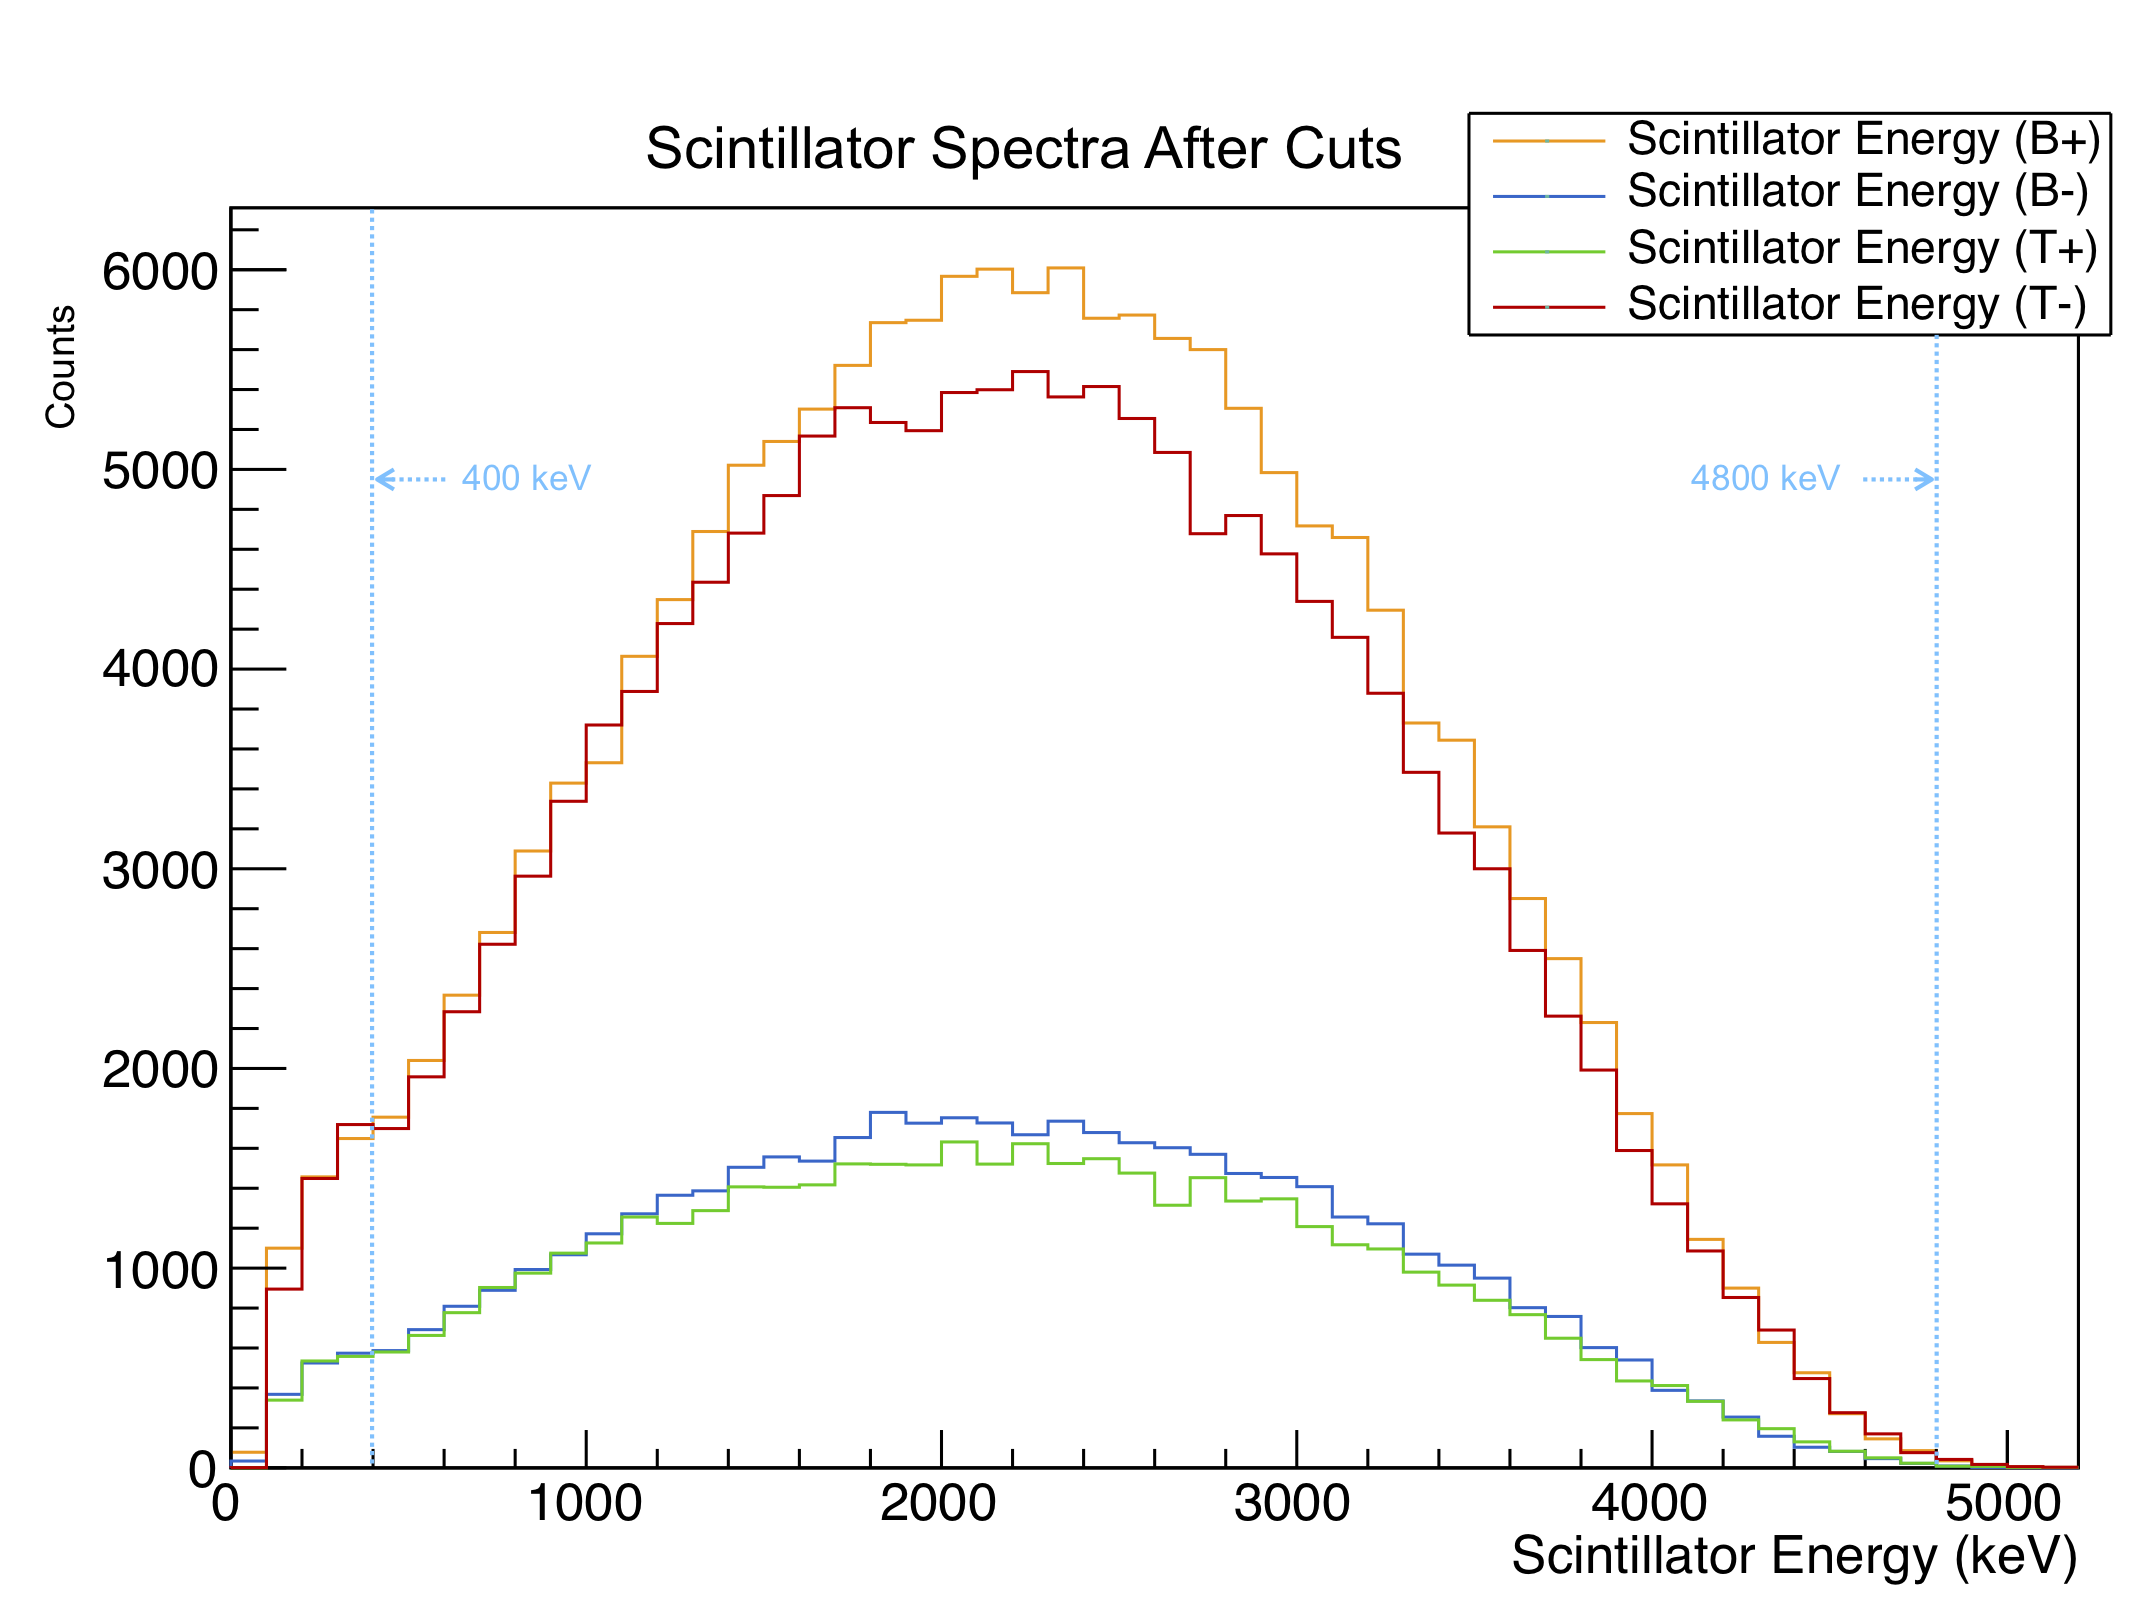
\includegraphics[width=.999\linewidth]
	{Figures/experimental_scintspectra_lin.png}
	\caption[Experimental Scintillator Spectra]{Experimental Scintillator Spectra, for both detectors in both polarization states.  These spectra are what remain after all cuts have been taken.  All runsets are included.}	
	\label{fig:scintspectra}
\end{figure}



\begin{figure}[h!!!!tb]
	\centering
	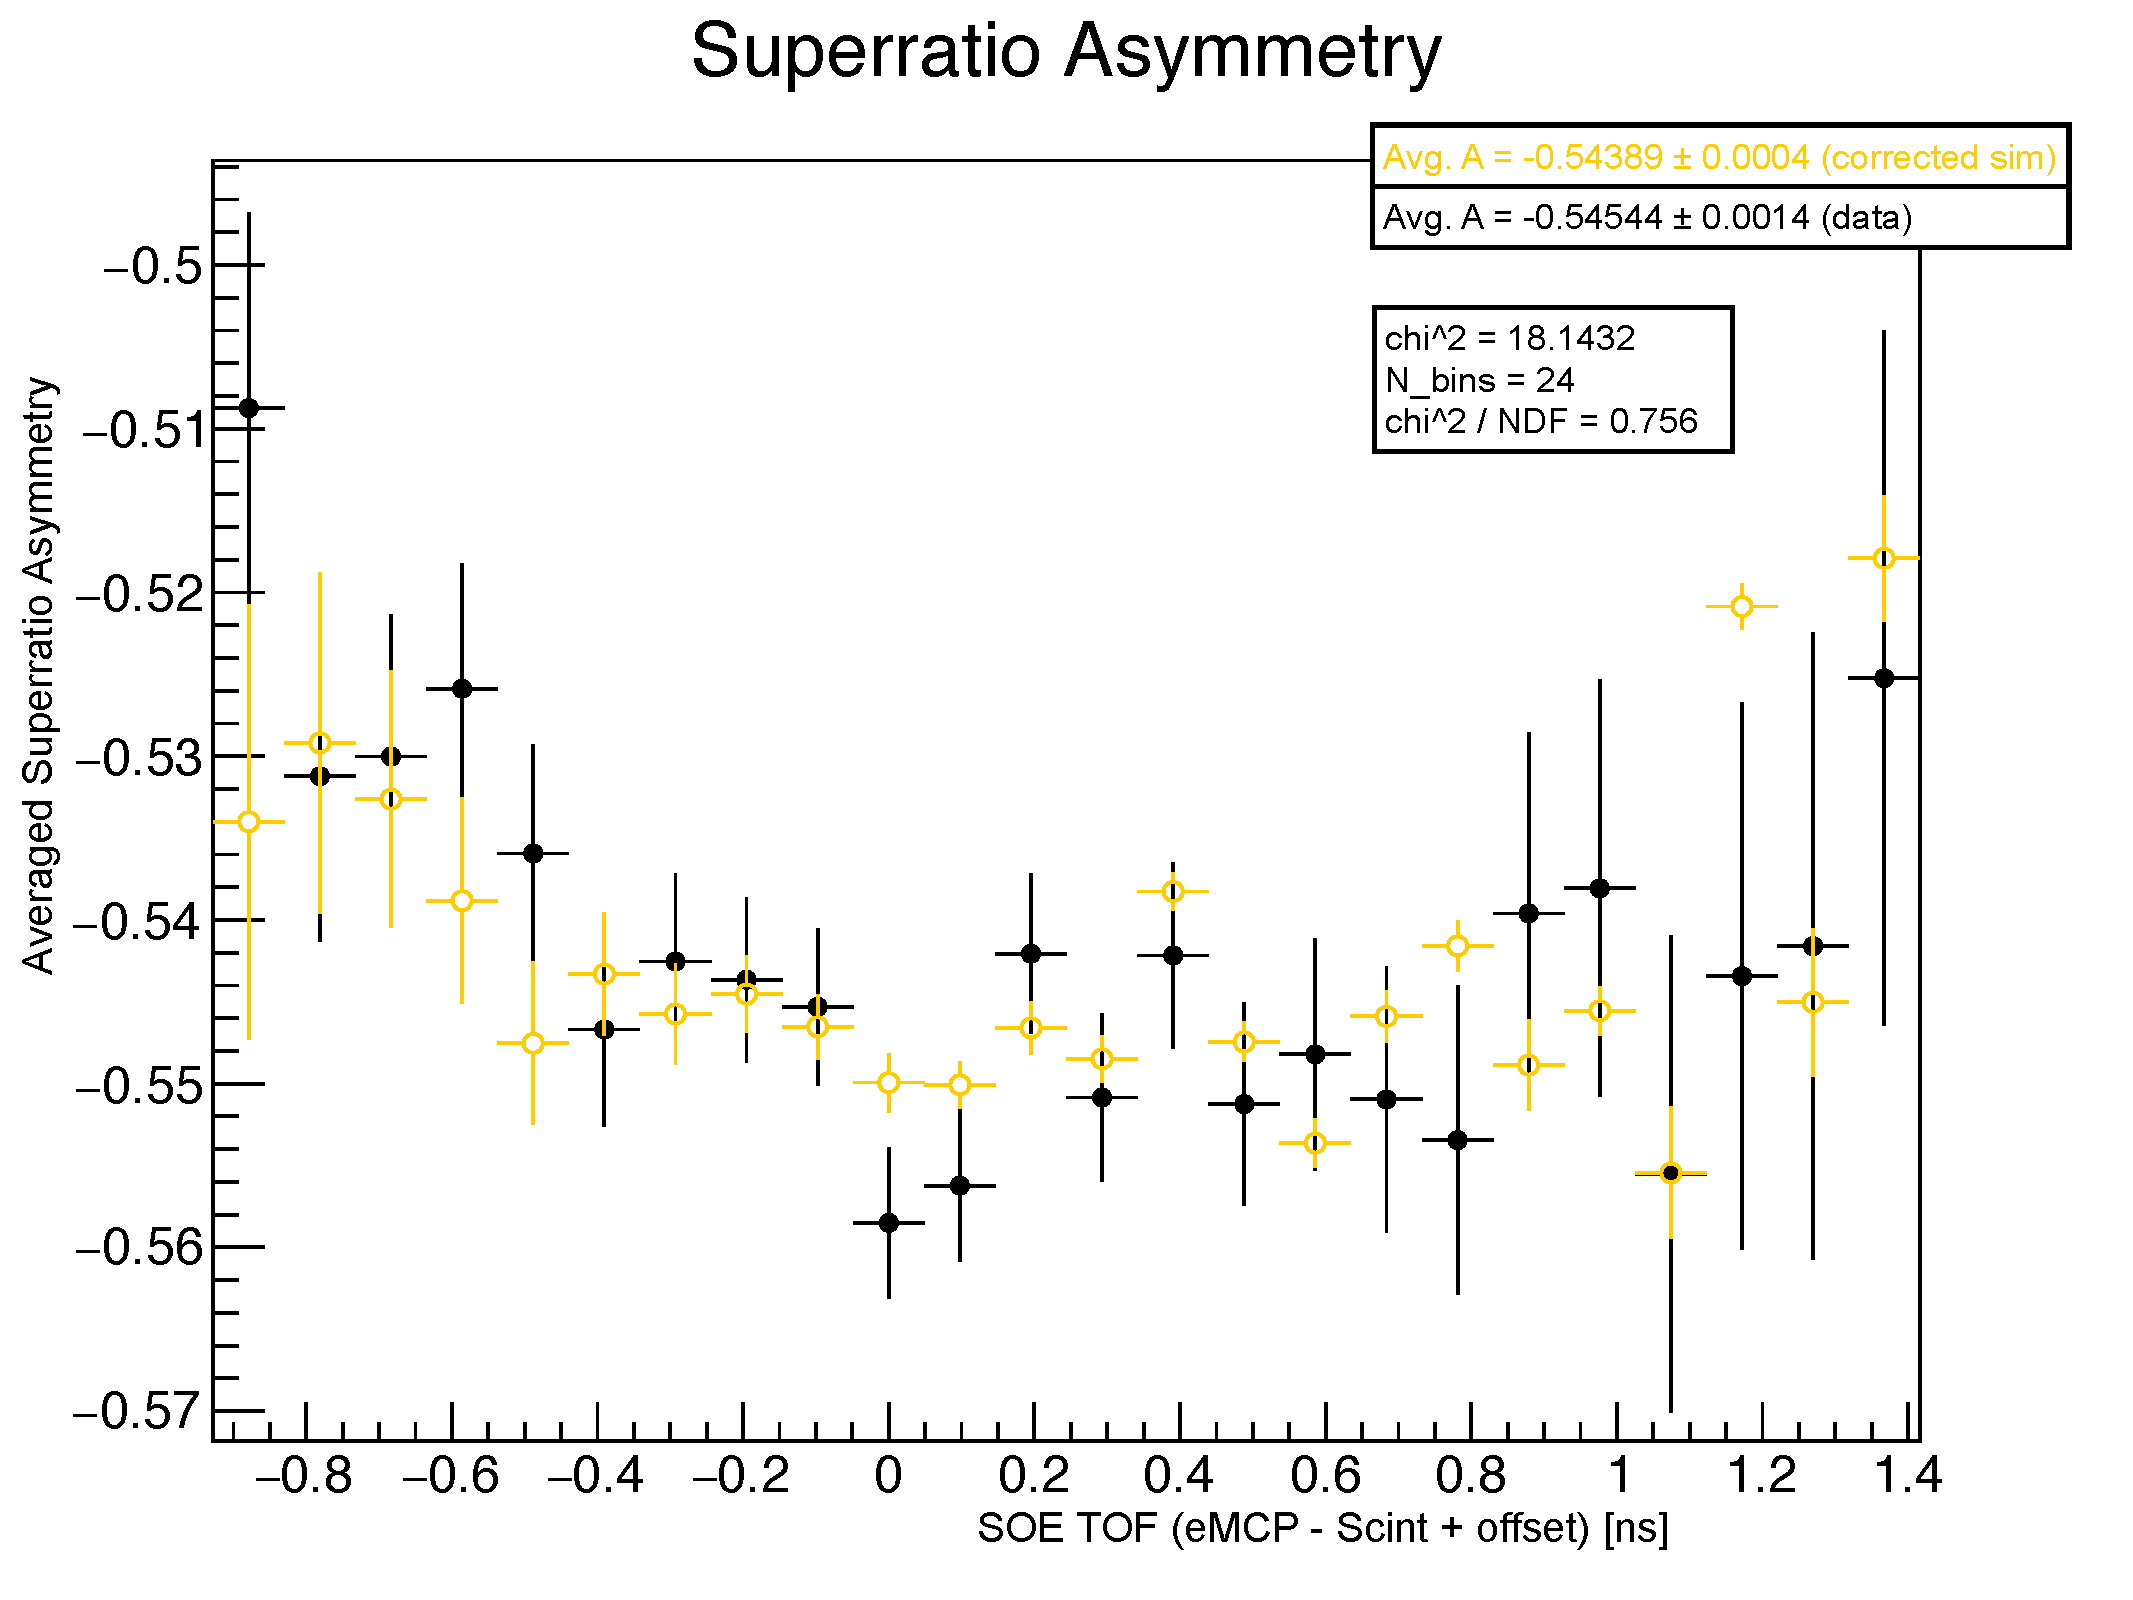
\includegraphics[width=.999\linewidth]
	{Figures/asymmetry_by_tof.pdf}
	\note{I think I want this picture to go in some other section.}
	\caption{The superratio asymmetry, averaged over all scintillator energies between 400-4800 keV, is used to compare the experimental data and simulated TOF model as a proxy for the quality of the model to estimate the background.  All other cuts have been applied.}	
	\label{fig:asymmetry_by_tof}
\end{figure}


%\section{Bullet Points!}
%Right, so.  Here's (more of) how I processed the data into an answer.  In bullet point form, so I don't forget stuff while I'm obsessively trying to phrase everything well.  
%\newline
%
%With the Data:
%\begin{itemize}
%%	\item \greycomment{Lower-level data cleaning.  Discard events during parts of the duty cycle when atoms weren't polarized.  Discard events near a recorded spark time. Discard events when the photoionization laser fires.  Discard events when the LED pulser used to calibrate the scintillators fires.}
%%	\item \greycomment{Split up runs into sets, to account for changing experimental conditions.  Possibly I should list what the differences between runs were somewhere.  But not in this section.  OTOH, ...maybe?}
%	%
%%	\item Make some more careful cuts to clean the data.  
%	%	\begin{itemize}
%%		\item \greycomment{Discard events without a ``good'' DSSD hit.  Eliminates vast majority of background 511s.  Necessitates having a definition of what a ``good'' DSSD hit is.  It's subtle enough that we'll want to leave some part of this definition of ``good'' to be varied as a systematic effect.  Notably, we consider energy agreement for each hit pixel, individual strip SNR, and overall DSSD energy threshold.  Also, hit radius w.r.t. center of detector.  This is a lot of stuff, all implemented by Ben -- and it needs to be done fairly early on in data processing in order to keep processing times for everything else manageable.  }
%		\item Discard events where SOE-Beta TOF falls outside a certain range.  Necessitates picking a ``good'' range.  The precise definition of ``good'' is varied as a systematic.  
%		\item \greycomment{There was a scintillator timing walk correction before taking the SOE-Beta TOF cut.}
%		\item \greycomment{Before the scintillator walk correction, there was the thing where the data was re-processed using the leading edge pulse rather than the trailing edge pulse.  Makes it cleaner.  Ben just got stuck with the trailing edge.}
%		\item \greycomment{Could have implemented an eMCP hit *position* requirement, but that kills too many stats.  It's like a factor of two.}
%	%	\end{itemize}
%\end{itemize}






